%%%%%%%%%%%%%%%%%%%%%%%%%%%%%%%%%%%%%%%%%%%%%%%%%%%%%%%%%%%%%%%%%%%%%%%%%%%%%%%%%%%%%%%%%%
%                                     SETTINGS                                           %
%%%%%%%%%%%%%%%%%%%%%%%%%%%%%%%%%%%%%%%%%%%%%%%%%%%%%%%%%%%%%%%%%%%%%%%%%%%%%%%%%%%%%%%%%%
\documentclass[aspectratio=169, t]{beamer}

\usepackage{amsmath,amssymb}
\usepackage{graphicx}
\usepackage{subcaption}
\usepackage{standalone}
\usepackage[makeroom]{cancel}
\usepackage{appendixnumberbeamer}
\usepackage{hyperref}
\usepackage{booktabs}
\usepackage{xcolor}
\usepackage{units}

\graphicspath{{../../../analysis/}}

\usetheme{default}

\setbeamertemplate{itemize items}[circle]
\setbeamertemplate{footline}[frame number]
\setbeamertemplate{navigation symbols}{}

\usepackage[backend = bibtex,
			style = authoryear,
			maxnames = 5,
			maxcitenames = 3,
			doi = false,
			eprint = false]{biblatex}
\addbibresource{../biblio.bib}

\definecolor{BgBlue}{rgb}{0.2,0.2,0.7}

\AtBeginSection[]{
	\begin{frame}
		\vfill
		\centering
		\begin{beamercolorbox}[sep=8pt,center,shadow=false,rounded=true]{title}
			\usebeamerfont{title}\insertsectionhead\par%
		\end{beamercolorbox}
		\vfill
	\end{frame}
}

\newtheorem{assu}{Assumption}
\newtheorem{prop}{Proposition}

\newcommand{\Z}{\mathcal{Z}}
\newcommand{\MW}{\underline{w}}

%%%%%%%%%%%%%%%%%%%%%%%%%%%%%%%%%%%%%%%%%%%%%%%%%%%%%%%%%%%%%%%%%%%%%%%%%%%%%%%%%%%%%%%%%%
%                                     TITLE                                              %
%%%%%%%%%%%%%%%%%%%%%%%%%%%%%%%%%%%%%%%%%%%%%%%%%%%%%%%%%%%%%%%%%%%%%%%%%%%%%%%%%%%%%%%%%%
\title{Do Minimum Wages Increase Rents?}
\subtitle{Evidence from US ZIP Codes Using High-Frequency Data}
\date{\today}
%\date{}
\author{Diego Gentile Passaro \and Santiago Hermo \and Gabriele Borg}
\institute{Brown University $ \quad\quad\quad $ Brown University $ \quad\quad\quad\quad\quad$  AWS}
% \titlegraphic{\hfill\includegraphics[height=1.5cm]{logo.pdf}}

%%%%%%%%%%%%%%%%%%%%%%%%%%%%%%%%%%%%%%%%%%%%%%%%%%%%%%%%%%%%%%%%%%%%%%%%%%%%%%%%%%%%%%%%%%
%                                         BODY                                           %
%%%%%%%%%%%%%%%%%%%%%%%%%%%%%%%%%%%%%%%%%%%%%%%%%%%%%%%%%%%%%%%%%%%%%%%%%%%%%%%%%%%%%%%%%%
\begin{document}
\maketitle


%%% Introduction %%%

\begin{frame}
	\frametitle{Motivation}
	
	Research on minimum wage (MW) has mostly focused on employment.
	% States: people work and reside under same MW.
	
	\vspace{1.5mm}

	However, as MW policies are \textit{place-based}, so one should expect broader effects 
	in the local economy:
	\begin{enumerate}[$\Rightarrow$]
		\item Housing market.
	\end{enumerate}

	\pause
	\vspace{3mm}
	\textbf{Prediction from theory}
	
    A canonical version of the (Muth-Mills) monocentric city model suggests that income increases will 
    pass-through 1:1 to rents \parencite{Brueckner1987}.  
    	\begin{enumerate}[$\Rightarrow$]
		\item We are not aware of empirical estimates of that pass-through!
	\end{enumerate}
\end{frame}

\begin{frame}
	\frametitle{This paper}
	We investigate the short term effects of MW policies on rents in the US:
	\begin{itemize}
		\vspace{.5mm} \item Accounting for spatial spillovers, we estimate 
		elasticity of median rents to workplace and residence MWs.
		\vspace{.5mm} \item Estimate pass-through of MW increases to rents.
	\end{itemize}
	
	\vspace{3mm}
	\pause
	To do so, we:
	\begin{itemize}
    	\vspace{.5mm} \item Exploit high-frequency (monthly) high-resolution 
    	(ZIP Code) rents data from Zillow.
    	\vspace{.5mm} \item Leverage timing and spatial variation in MW changes 
    	\textit{within} metropolitan areas.
    	\vspace{.5mm} \item Propose a novel model-based measure of exposure to MW changes based on 
    	commuting shares.
	\end{itemize}
\end{frame}

\begin{frame}
	\frametitle{Comparative statics intuition}
    
    \vspace{3mm}
    
	Think of a metropolitan area, and a MW increase in the business district (CBD). 
	
	\vspace{3mm}
	
    \textbf{Partial equilibrium: short term}
	\begin{itemize}
		\vspace{.5mm} \item Firms producing in the CBD will pay a higher wage. Income redistribution 
		from firms to low income workers.
		\vspace{.5mm} \item Income changes are heterogeneous across space because people work 
		and reside in different locations.
		\vspace{.5mm} \item Housing is a normal good. Housing demand in some areas increases 
		and landlords charge a higher rent.
	\end{itemize}

	\pause
	\vspace{3mm}
	\textbf{General equilibrium: long term} (Not this paper!)
	\begin{itemize}
	\vspace{.5mm} \item People change residence and workplace locations (sorting).
	\vspace{.5mm} \item Developers build more houses (supply response).
\end{itemize}
\end{frame}

\begin{frame}
\frametitle{A motivating example}
    \begin{columns}
        \begin{column}{0.44\textwidth}
            \vspace{-8mm}
            \begin{figure}
                \centering
                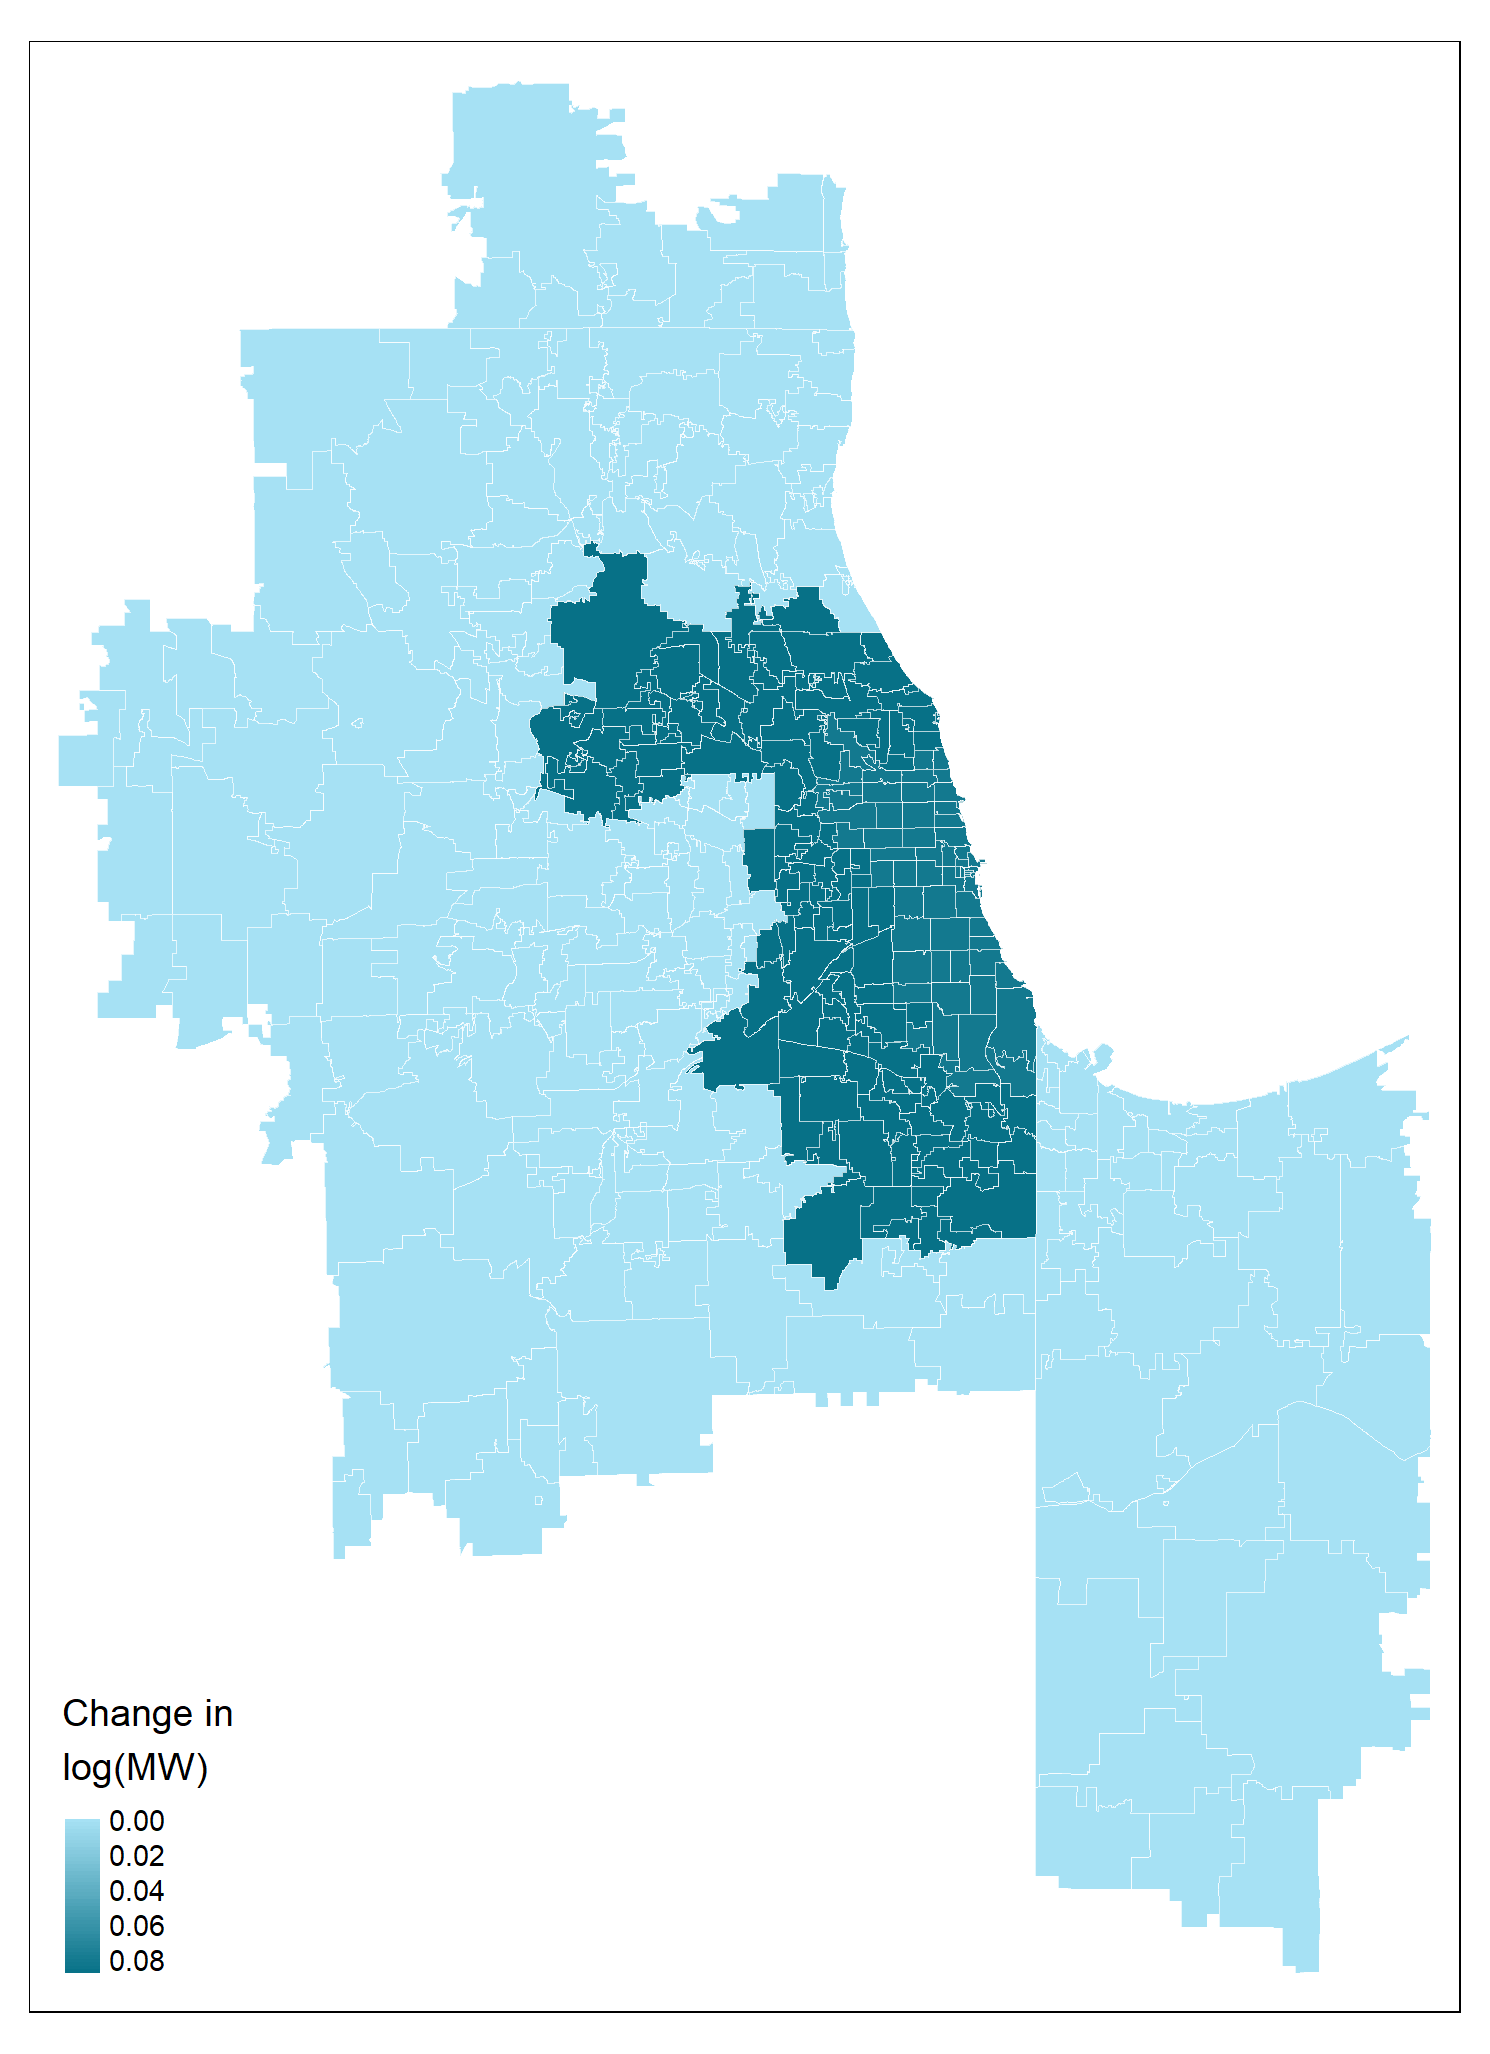
\includegraphics[scale = 0.38]{maps_events/output/chicago_2019-6_actual_mw.png}
            \end{figure}   
        \end{column}
        \begin{column}{0.56\textwidth}
            \begin{itemize}
                \item Cook County, IL, raised the statutory MW from \$12 to \$13 in July 2019. In the state of 
                Illinois the statutory MW is \$8.25 since 2010, while the federal one is of \$7.25 since 2009.
                \vspace{2mm}
                \pause
                \item A (naive) regression model of changes in rents on changes in MW's will imply that rents 
                can only be affected in Cook County.
                \vspace{2mm}
                \pause
                \item However, MW workers in Cook County may also live elsewhere in the 
                Chicago metropolitan area. $\to$ We need to take the commuting structure into account! 
            \end{itemize}
        \end{column}
    \end{columns}
\end{frame}

\begin{frame}
\frametitle{A novel model-based measure of access to MW's}

        For ZIP code $i$, and month $t$ we define it as:
	$$
	\underline{w}^{\text{exp}}_{it} = 
	\sum_{z \in \mathbb{Z}_i} \pi_{i z} \ln \underline{w}_{zt} \ ,
	$$
	%% IMPORTANT: We average the log of the MW! (Not log the average)
	\vspace{-2.5mm}
	where
	\vspace{1mm}
	\begin{itemize} \small
		\item $\mathbb{Z}_i$ are workplace locations of $i$'s residents, and
		\item $\pi_{i z} = \frac{L_{i z}}{L_i}$ is the share of $i$'s residents who work 
		in $z$.
	\end{itemize}
\end{frame}

\begin{frame}[label = chi_example]
\frametitle{A motivating example (Continuation)}
    \vspace{-6mm}
    \begin{columns}
        \begin{column}{0.50\textwidth}
            \vspace{-4mm}
            \begin{figure}
                \centering
                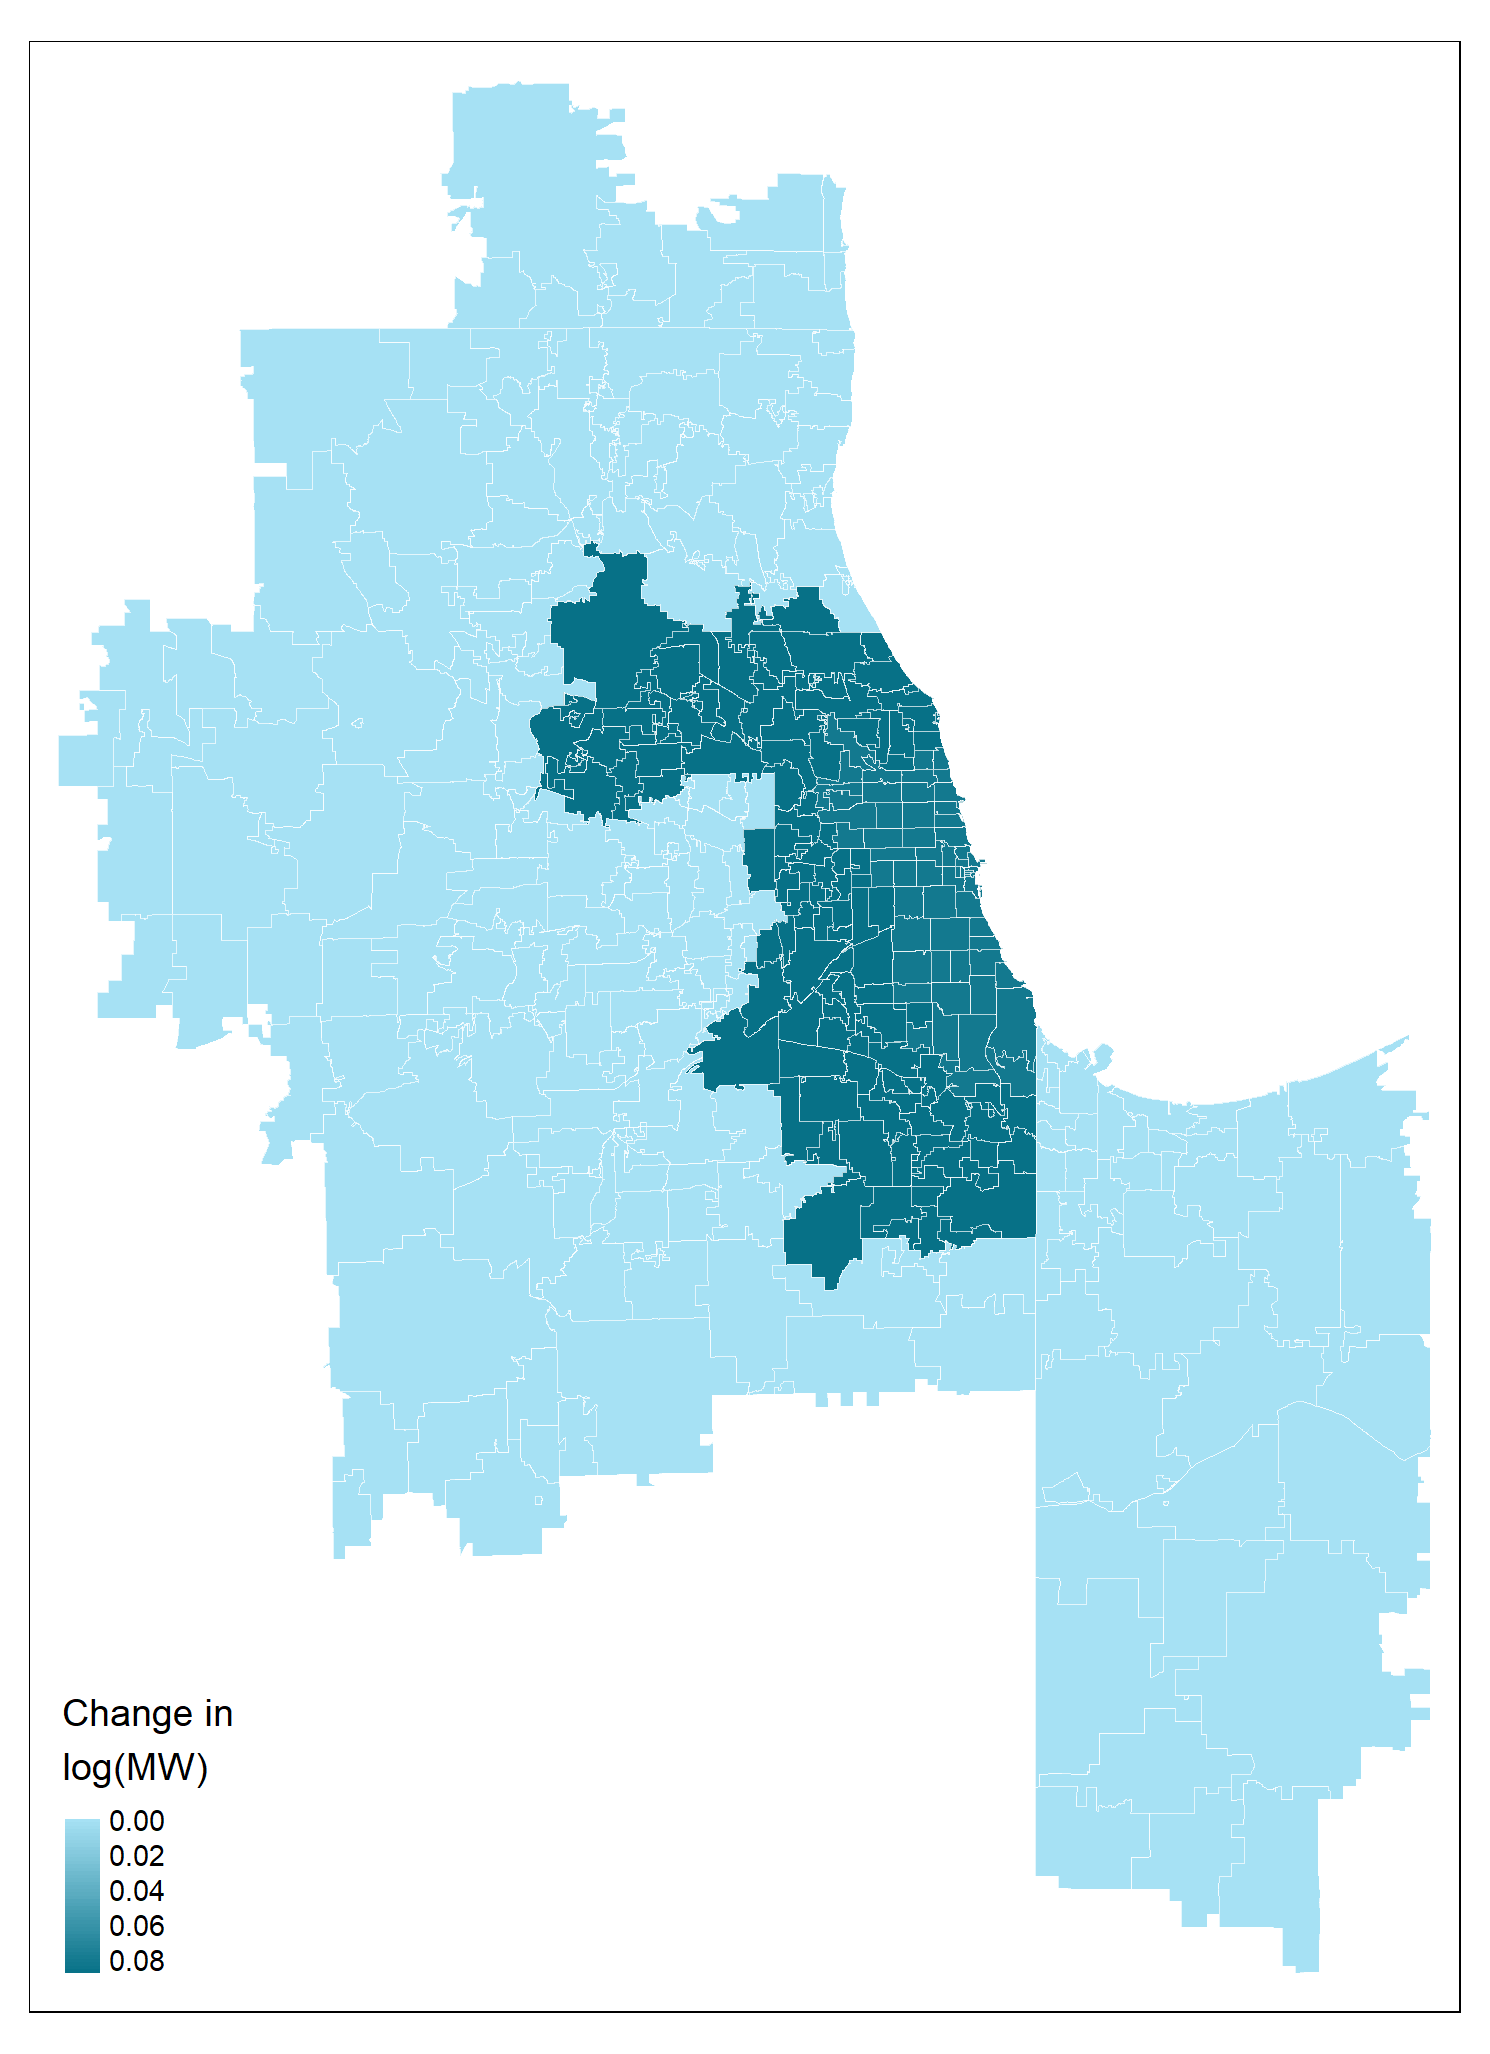
\includegraphics[scale = 0.36]{maps_events/output/chicago_2019-6_actual_mw.png}
            \end{figure}   
        \end{column}
        \begin{column}{0.50\textwidth}
            \vspace{-4mm}
            \begin{figure}
                \centering
                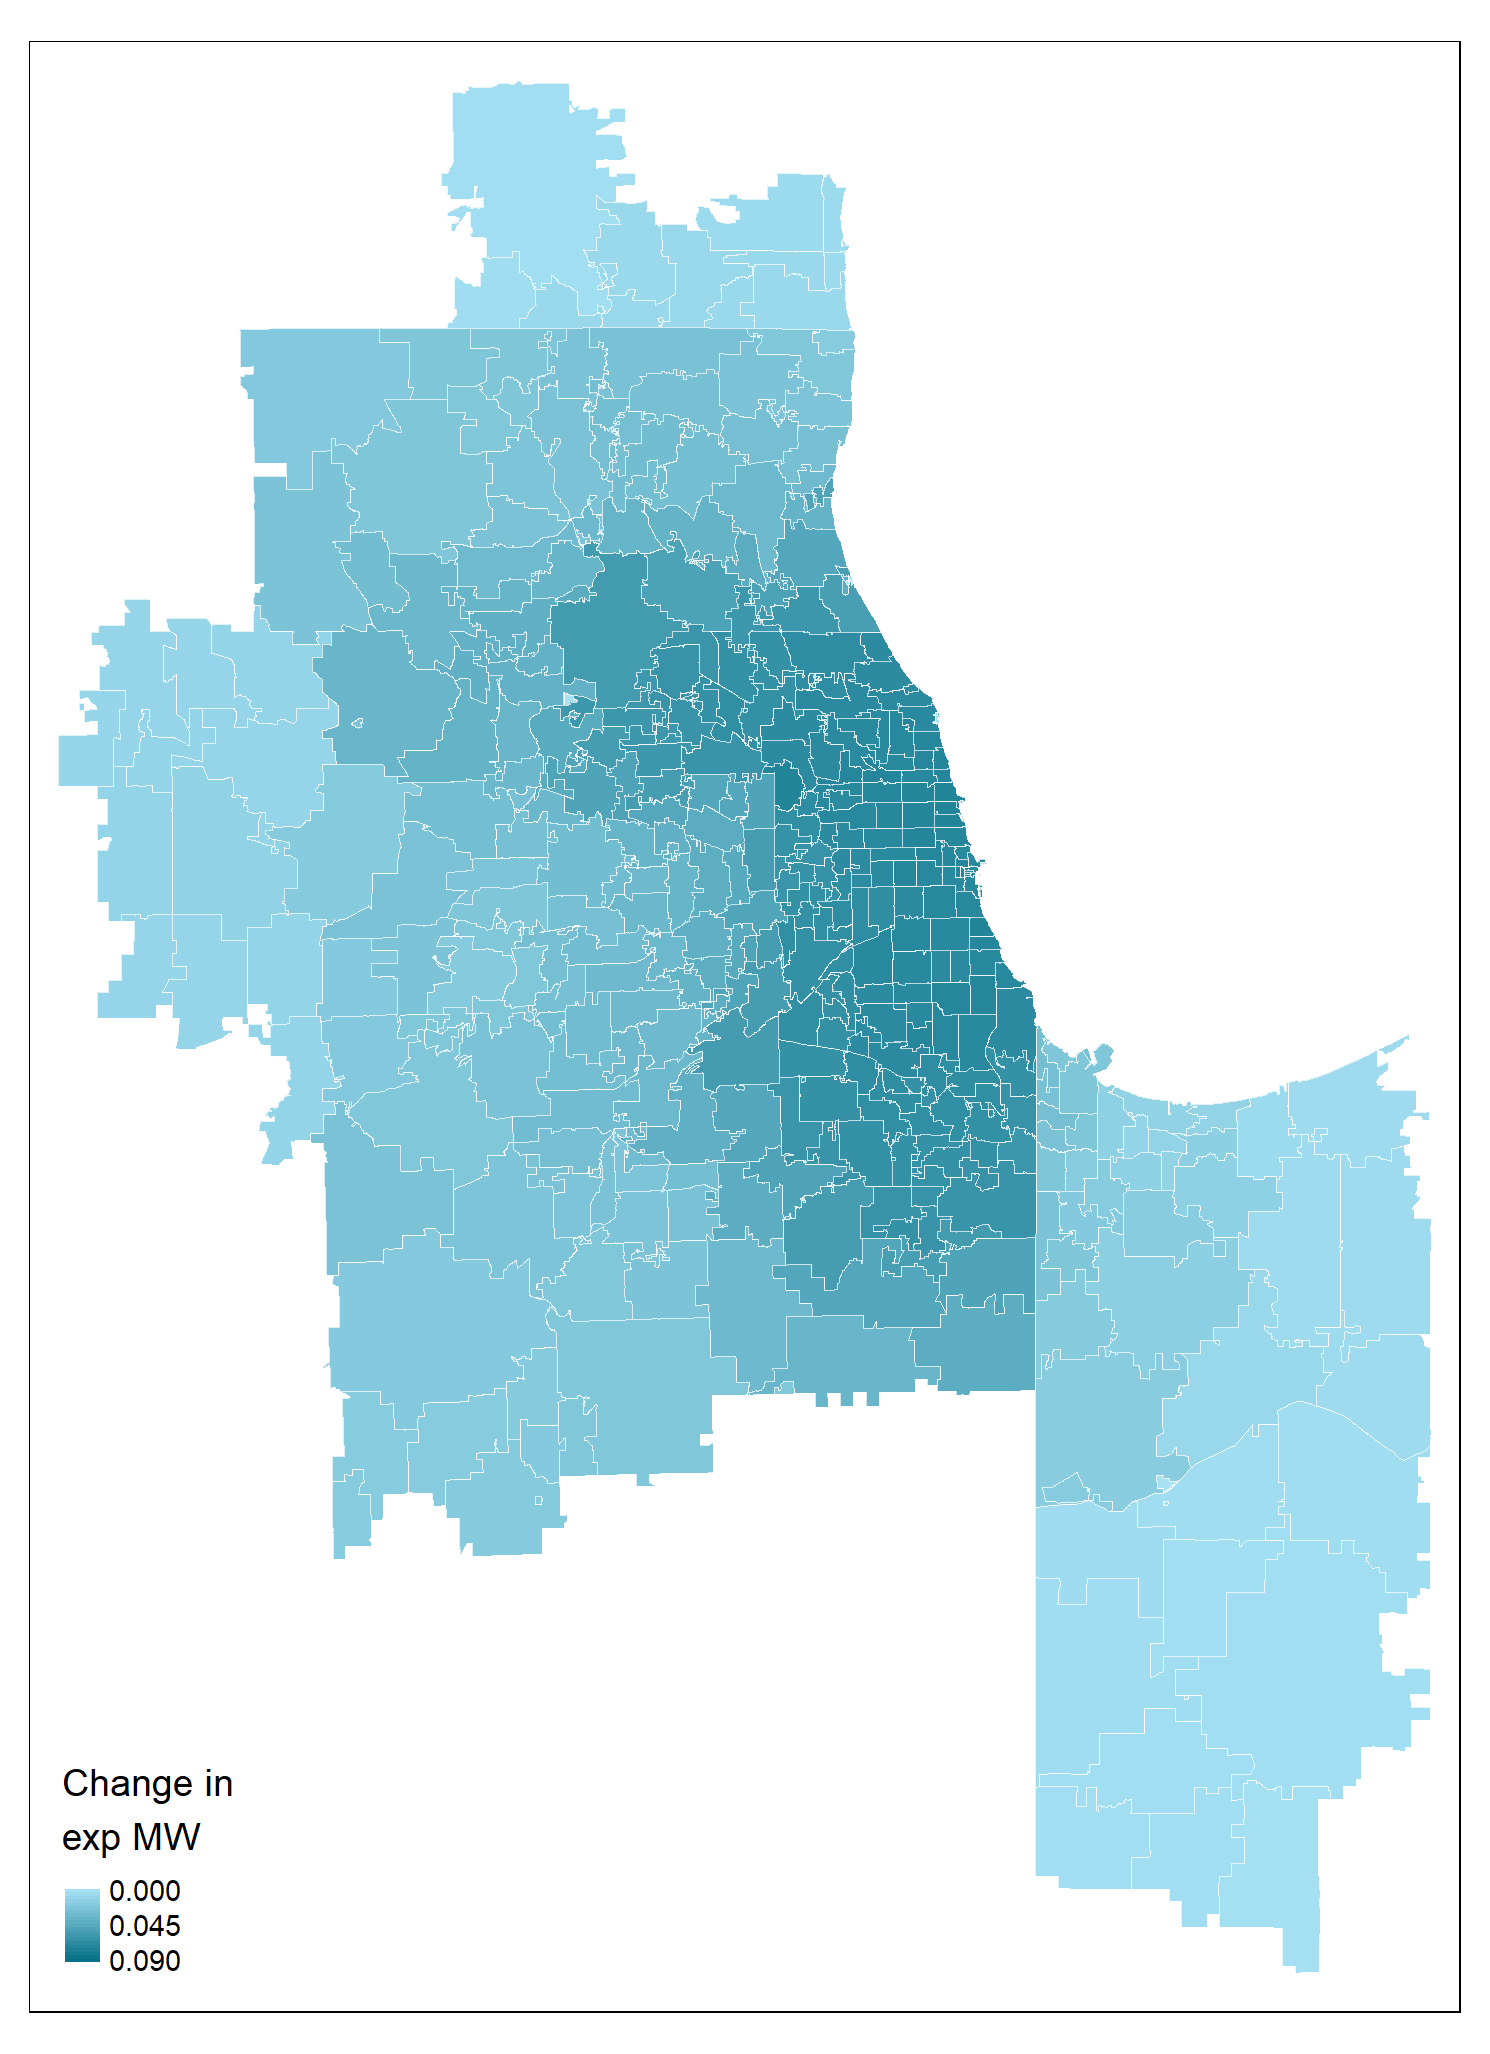
\includegraphics[scale = 0.36]{maps_events/output/chicago2019-6_exp_mw.png}
            \end{figure}   
        \end{column}
    \end{columns}
    \hspace{6mm}
    \hyperlink{nyc_example}{\beamerbutton{Example NYC}}    
    \hyperlink{seattle_example}{\beamerbutton{Example Seattle}}
    \hyperlink{bay_example}{\beamerbutton{Example Bay Area}}
    \hyperlink{san_diego_example}{\beamerbutton{Example San Diego}}
    \hyperlink{kc_example}{\beamerbutton{Example Kansas City}}
\end{frame}

\begin{frame}
	\frametitle{Outline for Today}
	\tableofcontents[hideallsubsections]
\end{frame}

\section{A Partial Equilibrium Model of the Local Rental Markets}

\begin{frame}
    \frametitle{Overview}
    
    	Goals of the model:
	\begin{itemize}
		\item Stylized answer to: what is the short-term effect of MW changes in rent prices?
		\item Motivate a new access to MW measure: the experienced MW.
		\item Emphasize why one may expect residence and worker MWs to have different effects on the housing market.
		\item Motivate our empirical strategy: use commuting patterns to account for spatial
		spillovers of MW policies.
	\end{itemize}
	
	\pause
	\vspace{2mm}
	The model is \textit{not} intended to:
	\begin{itemize}
		\item Describe within-city residential sorting.
		\item Describe the local labor markets.
		\item Describe the local goods markets.
		\item Perform general equilibrium welfare analysis of MW policies.
	\end{itemize}
\end{frame}

\begin{frame}
    \frametitle{Setup}
    
    Static rental market of some residence ZIP code $i$ embedded in a larger geography 
    $\Z$ with finite number of ZIP codes.    
    \begin{itemize}
		\item Workers with residence $i$ may work in some other ZIP code $z\in\Z(i)$, where 
		$\Z(i)\subseteq\Z$.

		\pause
		\vspace{2mm}
		\item Exogenous and fixed $L_{iz}$ that denotes the measure of $i$'s residents who work in $z$.
		\begin{itemize}
			\item Measure of residents in $i$: $L_i = \sum_{z \in \Z(i)} L_{iz}$
			\item Measure of workers in $z$: $L_z = \sum_{i \in \Z(i)} L_{iz}$ 
		\end{itemize}
		
		\item Commuter shares: $\pi_{iz} = \frac{L_{iz}}{L_i}$
	
		\pause
		\item Binding minimum wages: $\{\MW_z\}_{z\in\Z}$
		
		\pause
		\vspace{2mm}
		\item $H_{i z} (r_i, \MW_i, \MW_z)$: housing demand, where $r_i$ 
		represents housing rents.
		
		\pause
		\vspace{2mm}
		\item $D_i \left(r_i \right)$: supply of square feet in $i$, which is increasing in $r_i$.

	\end{itemize}
\end{frame}

\begin{frame}
    \frametitle{Housing Demand}
   
\begin{assu}[Housing demand]\label{assu:housing_function}
    For all residence-workplace pairs, the housing demand function $h_{iz} (r_i, 	
    \MW_i, \MW_z)$ is:
    \begin{enumerate}
        \item continuously differentiable in its three arguments;
        \item decreasing in rental prices $r_i$;
        \item non-decreasing in workplace minimum wage $\MW_z$.
        \item non-increasing in residence minimum wage $\MW_i$;
    \end{enumerate}
    Furthermore, for at least one $z\in\Z(i)$, the inequalities in points (iii)
    and (iv) are strict.
\end{assu}
\end{frame}

\begin{frame}
    \frametitle{Discussion on 4.}
    
    %%% This slide we should discuss and change accordingly!
    
    \textbf{In words:} conditional on workplace MWs, residence MW may negatively affect disposable income
     and thus demand for housing.
     
     \pause 
     \vspace{2mm}

    We think that the interpretation underlying point 4. is plausible:
    \begin{itemize}
        \item Recent evidence by \textcite{MiyauchiEtAl2021} shows that individuals tend to consume 
        close to home. Households respond and are aware of price differentials in local consumption across neighborhoods.
        \item MWs have been shown to increase prices of local consumption 
        \parencite[e.g.,][]{AllegrettoReich2018, LeungForthcoming}.
    \end{itemize}

    \pause 
    \vspace{2mm}

    Potential microfoundation:
    \begin{itemize}
        \item If firms in $i$ that produce non-tradable local goods, use MW workers as an input, 
        then a MW increase will increase prices. Higher cost of non-tradables will translate into a 
        lower demand for housing if the substitution effect on local demand of housing is smaller than 
        the corresponding income effect. 
        \item A sufficient condition for that is that housing and local consumption are complements.
    \end{itemize}
\end{frame}

\subsection{Equilibrium and Comparative Statics}
\begin{frame}
	\frametitle{Equilibrium}
	
	The rental market of ZIP code $i$ is in equilibrium if
	
	$$\sum_{z\in\Z(i)} L_{iz} h_{iz} (r_i, \MW_i, \MW_z) = D_i(r_i) $$
	
    As housing demand functions are continuous and decreasing in rents, 
    under suitable regularity conditions there is a unique equilibrium in this market.%
    
    \vspace{2mm}

    We denote equilibrium rents as $r^*_i = f(\{\MW_i\}_{i\in\Z(i)})$.
	
	\vspace{5mm}
	\pause
	We are interested in the effects of MW policies on rents.
	\vspace{1mm}
	\begin{itemize} \small
		\item What is the effect of a change in the vector of MWs 
		$(\{d \MW_i\}_{i\in\Z(i)})'$ on equilibrium rents?
		\item Under what conditions can we represent those effects in a simple way?
	\end{itemize}
\end{frame}

\begin{frame}[label = prop_comp_stat]
    \frametitle{Comparative Statics}
    
    \begin{prop}[Comparative Statics]\label{prop:comparative_statics}
        Under the assumptions of:
        \begin{enumerate}
           \item Fixed of workers across workplace and residence pairs.
            \item housing demand equation satisfying Assumption \ref{assu:housing_function}, 
            \item continuously differentiable and increasing housing supply.
        \end{enumerate} 
        We have that:
        \begin{itemize}
            \item workplace-MW hikes increase rents.
            \item holding constant workplace-MW hikes, residence-MW hikes decrease rents.
        \end{itemize}
    \end{prop}
\end{frame}

\begin{frame}[label = proof_comp_stat]
\frametitle{Proof of Proposition (Comparative Statics)}

\begin{proof}
    Fully differentiate the market clearing condition with respect to $\ln r_i$ and 
    $\ln \MW_i$ for all $i\in\Z(i)$ and re-arrange terms to get:
    \begin{equation}\label{eq:diff_equilibrium}
        \Big(\eta_i - \sum_z \pi_{iz} \xi_{iz} \Big) d \ln r_i
        = 
        \sum_z \pi_{iz} \left(\epsilon_{iz}^i d \ln \MW_i 
                            + \epsilon_{iz}^z d \ln \MW_z \right) ,
    \end{equation}
    where:
    \begin{itemize}
        \item $\xi_{iz} = \frac{d h_{iz}}{d r_i} \frac{r_i}{\sum_z \pi_{iz} h_{iz}}$ is the 
        elasticity of housing demand at the average per-capita demand of ZIP code $i$
        \item  $\epsilon_{iz}^i = \frac{d h_{iz}}{d \MW_i} \frac{\MW_i}{\sum_z \pi_{iz} h_{iz}}$ and 
        $\epsilon_{iz}^z = \frac{d h_{iz}}{d \MW_z} \frac{\MW_z}{\sum_z \pi_{iz} h_{iz}}$ 
        are the elasticities of housing demand to workplace and residence MWs also at
         the average per-capita demand of ZIP code $i$
         \item $\eta_i = \frac{1}{L_i} \frac{d D_i}{d r_i} \frac{r_i}{D_i}$ is the elasticity 
         of housing supply in ZIP code $i$
    \end{itemize}
\end{proof}
\end{frame}

\begin{frame}
    \frametitle{Proof of Proposition (Comparative Statics) (Continuation)}
    
    Using that:
    \begin{itemize} 
        \item $\xi_{iz} < 0$ for at least some workplace
        \item $\epsilon_{iz}^i < 0$
        \item $\epsilon_{iz}^z > 0$
    \end{itemize}
    It follows from \eqref{eq:diff_equilibrium} that:
    \begin{enumerate}
        \item an increase in workplace MW unambiguously increases rents
        \item an increase in residence MW on rents is generally ambiguous 
        (as long as some residents of $i$ also work in $i$) as it is composed of a direct negative 
        effect and an indirect positive effect through changing the experienced MW. \footnote{The sign of the overall partial effect depends on the sign of 
    $\pi_{ii} \epsilon_{ii}^z + \sum_z \pi_{iz} \epsilon_{iz}^i$.}
        \item Holding constant workplace MWs, the effect of the residence MW is negative.
    \end{enumerate}    
\end{frame}

\begin{frame}[label = representation_prop]
    \frametitle{Representation}
    
\begin{prop}[Representation]\label{prop:representation}
    Under the assumption of constant elasticity of housing demand (across workplace locations)
    to workplace minimum wages we have that:
    \begin{itemize}
        \item We can write the change in log rents as a function of the change in two 
        MW-based measures: the \textbf{experienced log MW} and the \textbf{statutory log MW}.
    \end{itemize}
\end{prop}

\pause
\vspace{2mm}

\begin{proof}
    Set $\epsilon_{iz}^z = \epsilon_i^z$ for all $z\in\Z(i)$ 
    we can manipulate \eqref{eq:diff_equilibrium} to write:
    \begin{equation} \label{eq:theory_represenation}
        d \ln r_i = \beta_i \sum_i \pi_{iz} d\ln \MW_z + \gamma_i d \ln \MW_i
    \end{equation}
    where $\beta_i = \frac{\epsilon_{i}^z}{\eta_{i} - \sum_z \pi_{iz} \xi_{iz}}$ 
    and $\gamma_i = \frac{\sum_z \pi_{iz} \epsilon_{iz}^i}{\eta_{i} 
            - \sum_z \pi_{iz} \xi_{iz}}$.
\end{proof}
\end{frame}

\begin{frame}
\frametitle{Motivating our empirical Strategy}
Using Proposition (Comparative Statics), our Proposition (Representation) implies that:
\begin{itemize}
    \item The partial equilibrium effect of workplace MW, $\beta_i = \frac{\epsilon_{i}^z}{\eta_{i} - \sum_z \pi_{iz} \xi_{iz}} > 0$
    \item The partial equilibrium effect of residence MW, $\gamma_i = \frac{\sum_z \pi_{iz} \epsilon_{iz}^i}{\eta_{i} 
            - \sum_z \pi_{iz} \xi_{iz}} < 0$.
\end{itemize}

Therefore our model yields:
	\begin{equation} \label{eq:theory_represenation}
            d \ln r_i = \beta_i \sum_i \pi_{iz} d\ln \MW_z + \gamma_i d \ln \MW_i
        \end{equation}
        
We will estimate an empirical analog assuming (for today) homogenous effects.

\end{frame}

\section{Data}

%\subsection{Zillow}

\begin{frame}[label = zillow]
	\frametitle{Zillow Data}
	
	\begin{itemize}
		\item Leader online real estate and rental platform in the U.S. {\small (more 
		than 110 million homes and 170 million unique monthly users in 2019).}
		
		\vspace{2mm} \item
		Provides \textit{median} rents data at ZIP code, county, and state levels 
		at a monthly frequency for several housing categories.
		
		\pause
		\vspace{2mm} \item
		Use category single-family, condominium, and cooperative houses (SFCC):
		\begin{itemize}
			\item Most common housing type in the U.S.
			\item Most populated series in Zillow.
			%%\item Captures trends in metropolitan housing markets. 
			%%\hyperlink{zillow_safmr}{\beamerbutton{Comparison SAFMR}}
		\end{itemize}
		
		\pause
		\vspace{2mm} \item
		Limitation: Zillow sample is not random.
	\end{itemize}
\end{frame}

\begin{frame}
	\frametitle{Comparison between Zillow Sample and Population Density}
    \begin{figure}
    	\centering
	\vspace{10mm}
	\hspace{-23mm}
    	\begin{subfigure}{0.40\textwidth}
    		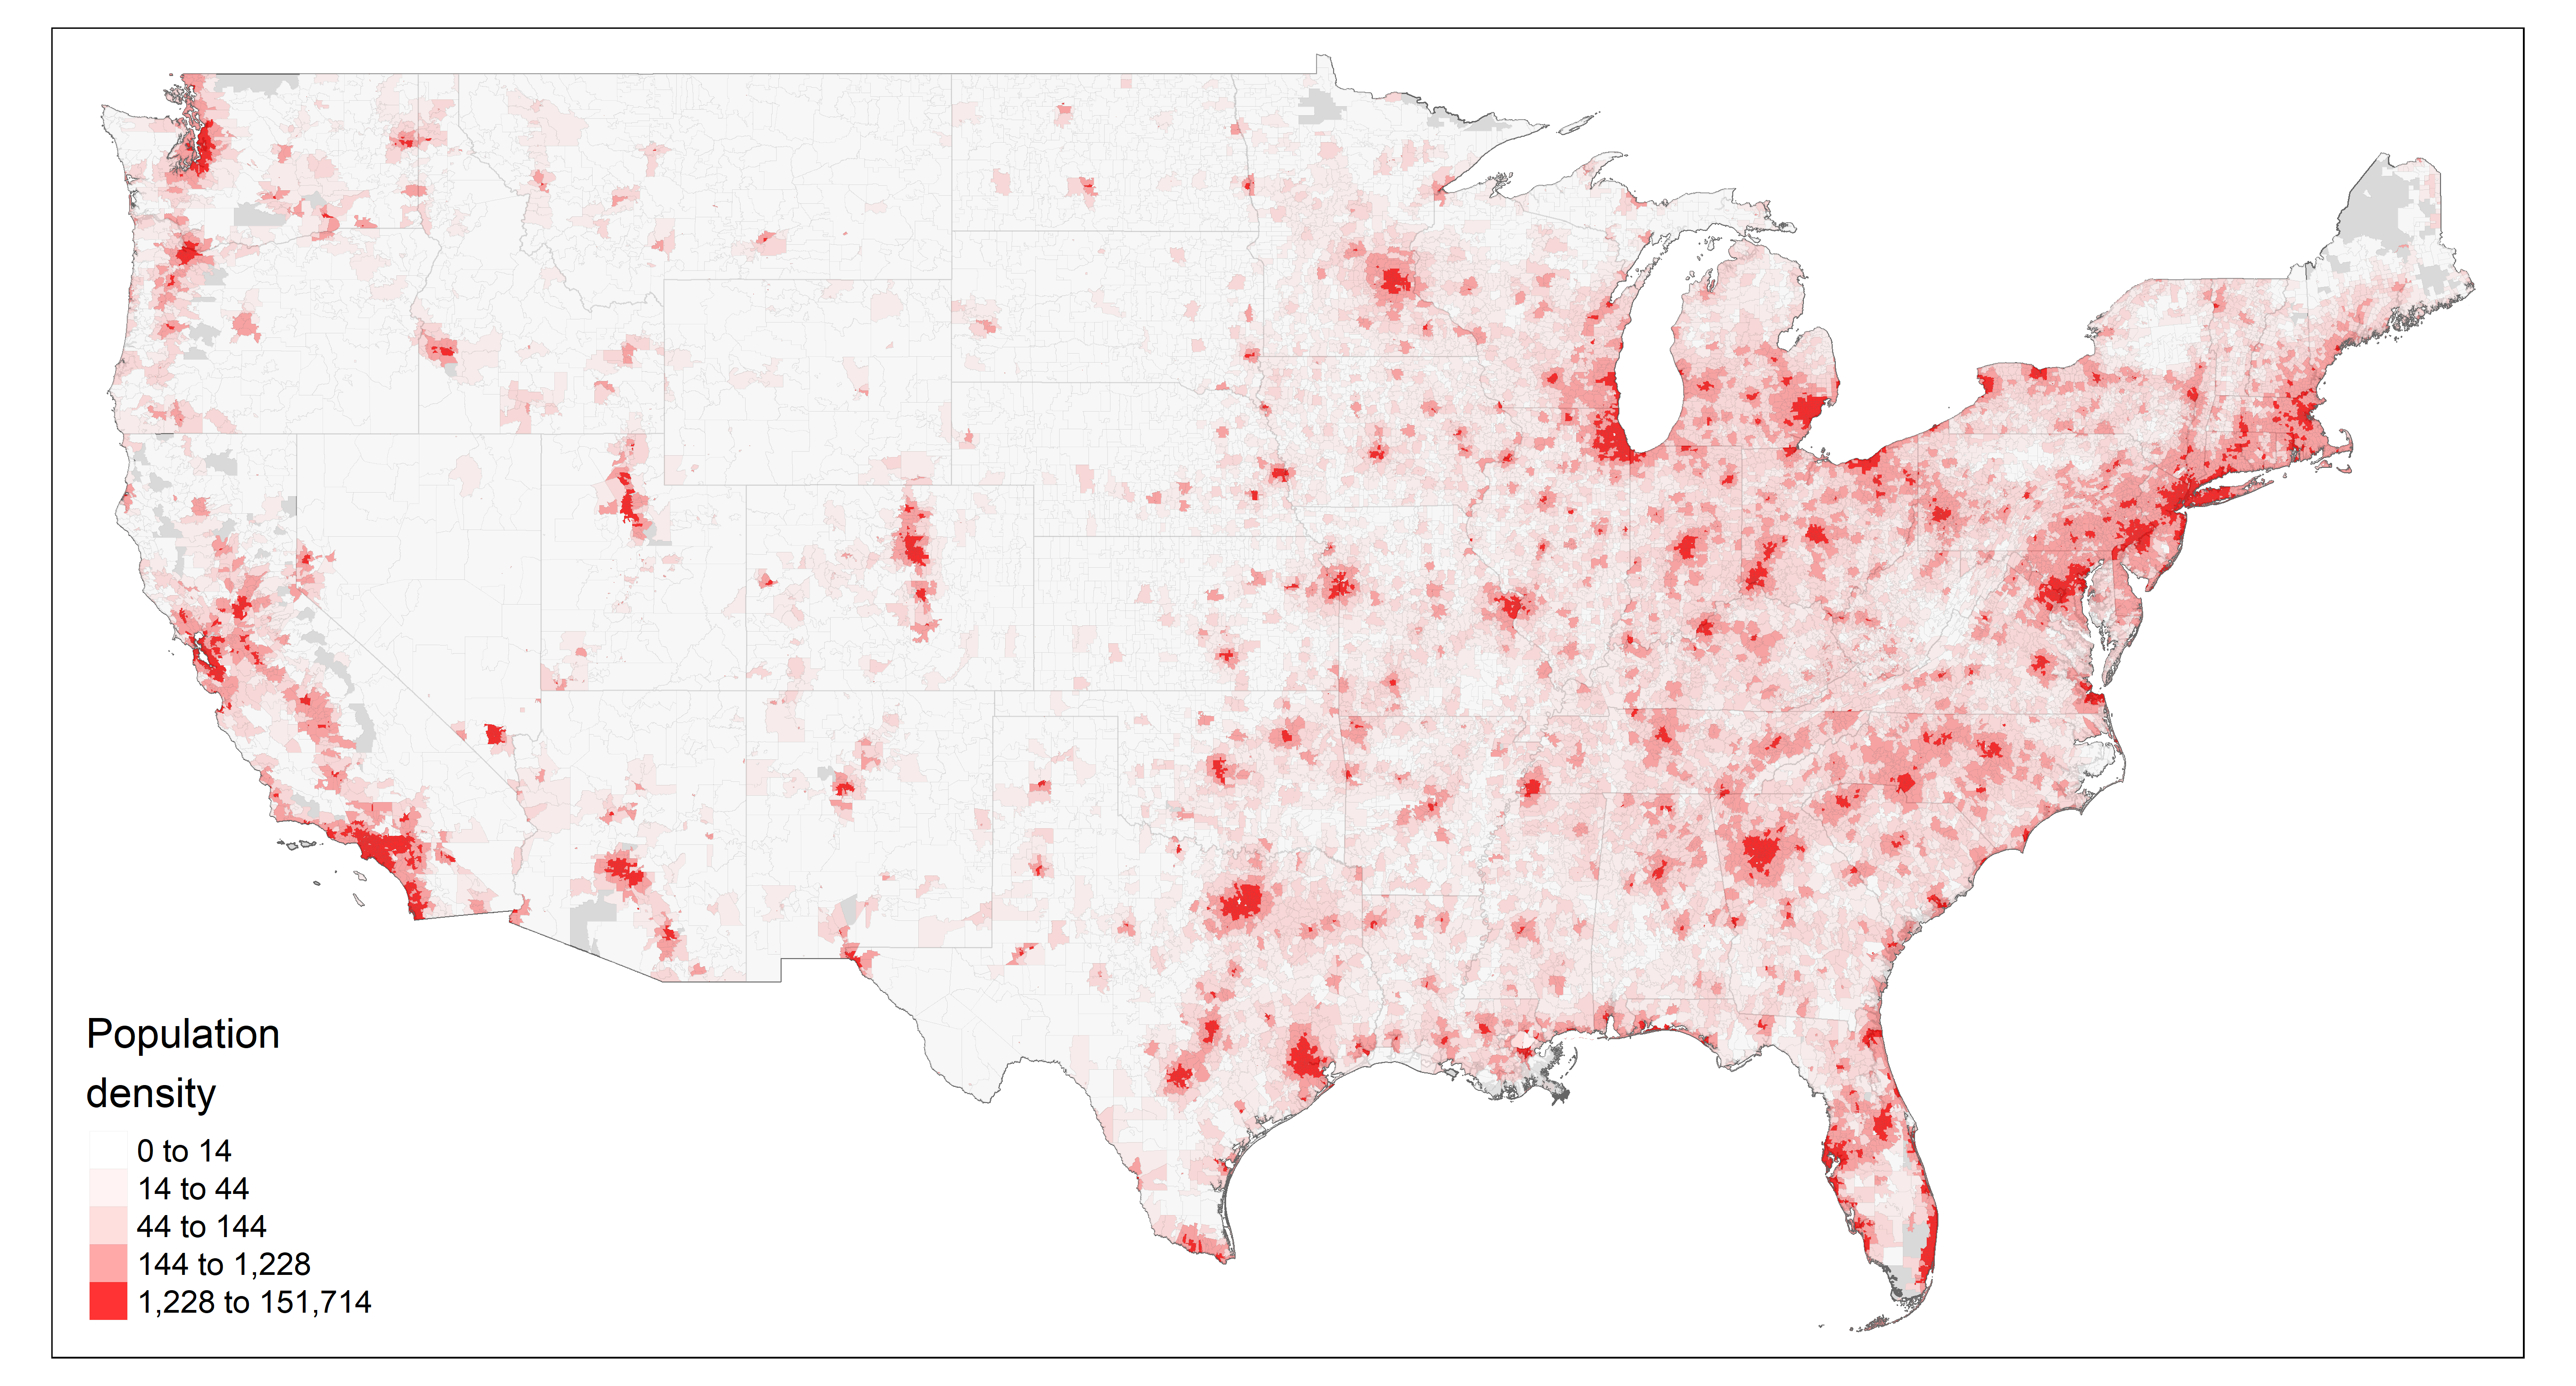
\includegraphics[scale = 0.32]{maps_US/output/USPS_zipcodes_pop_density.png}
    	\end{subfigure}%
	\quad\quad\quad\quad\quad\quad
        \begin{subfigure}{0.40\textwidth}
        	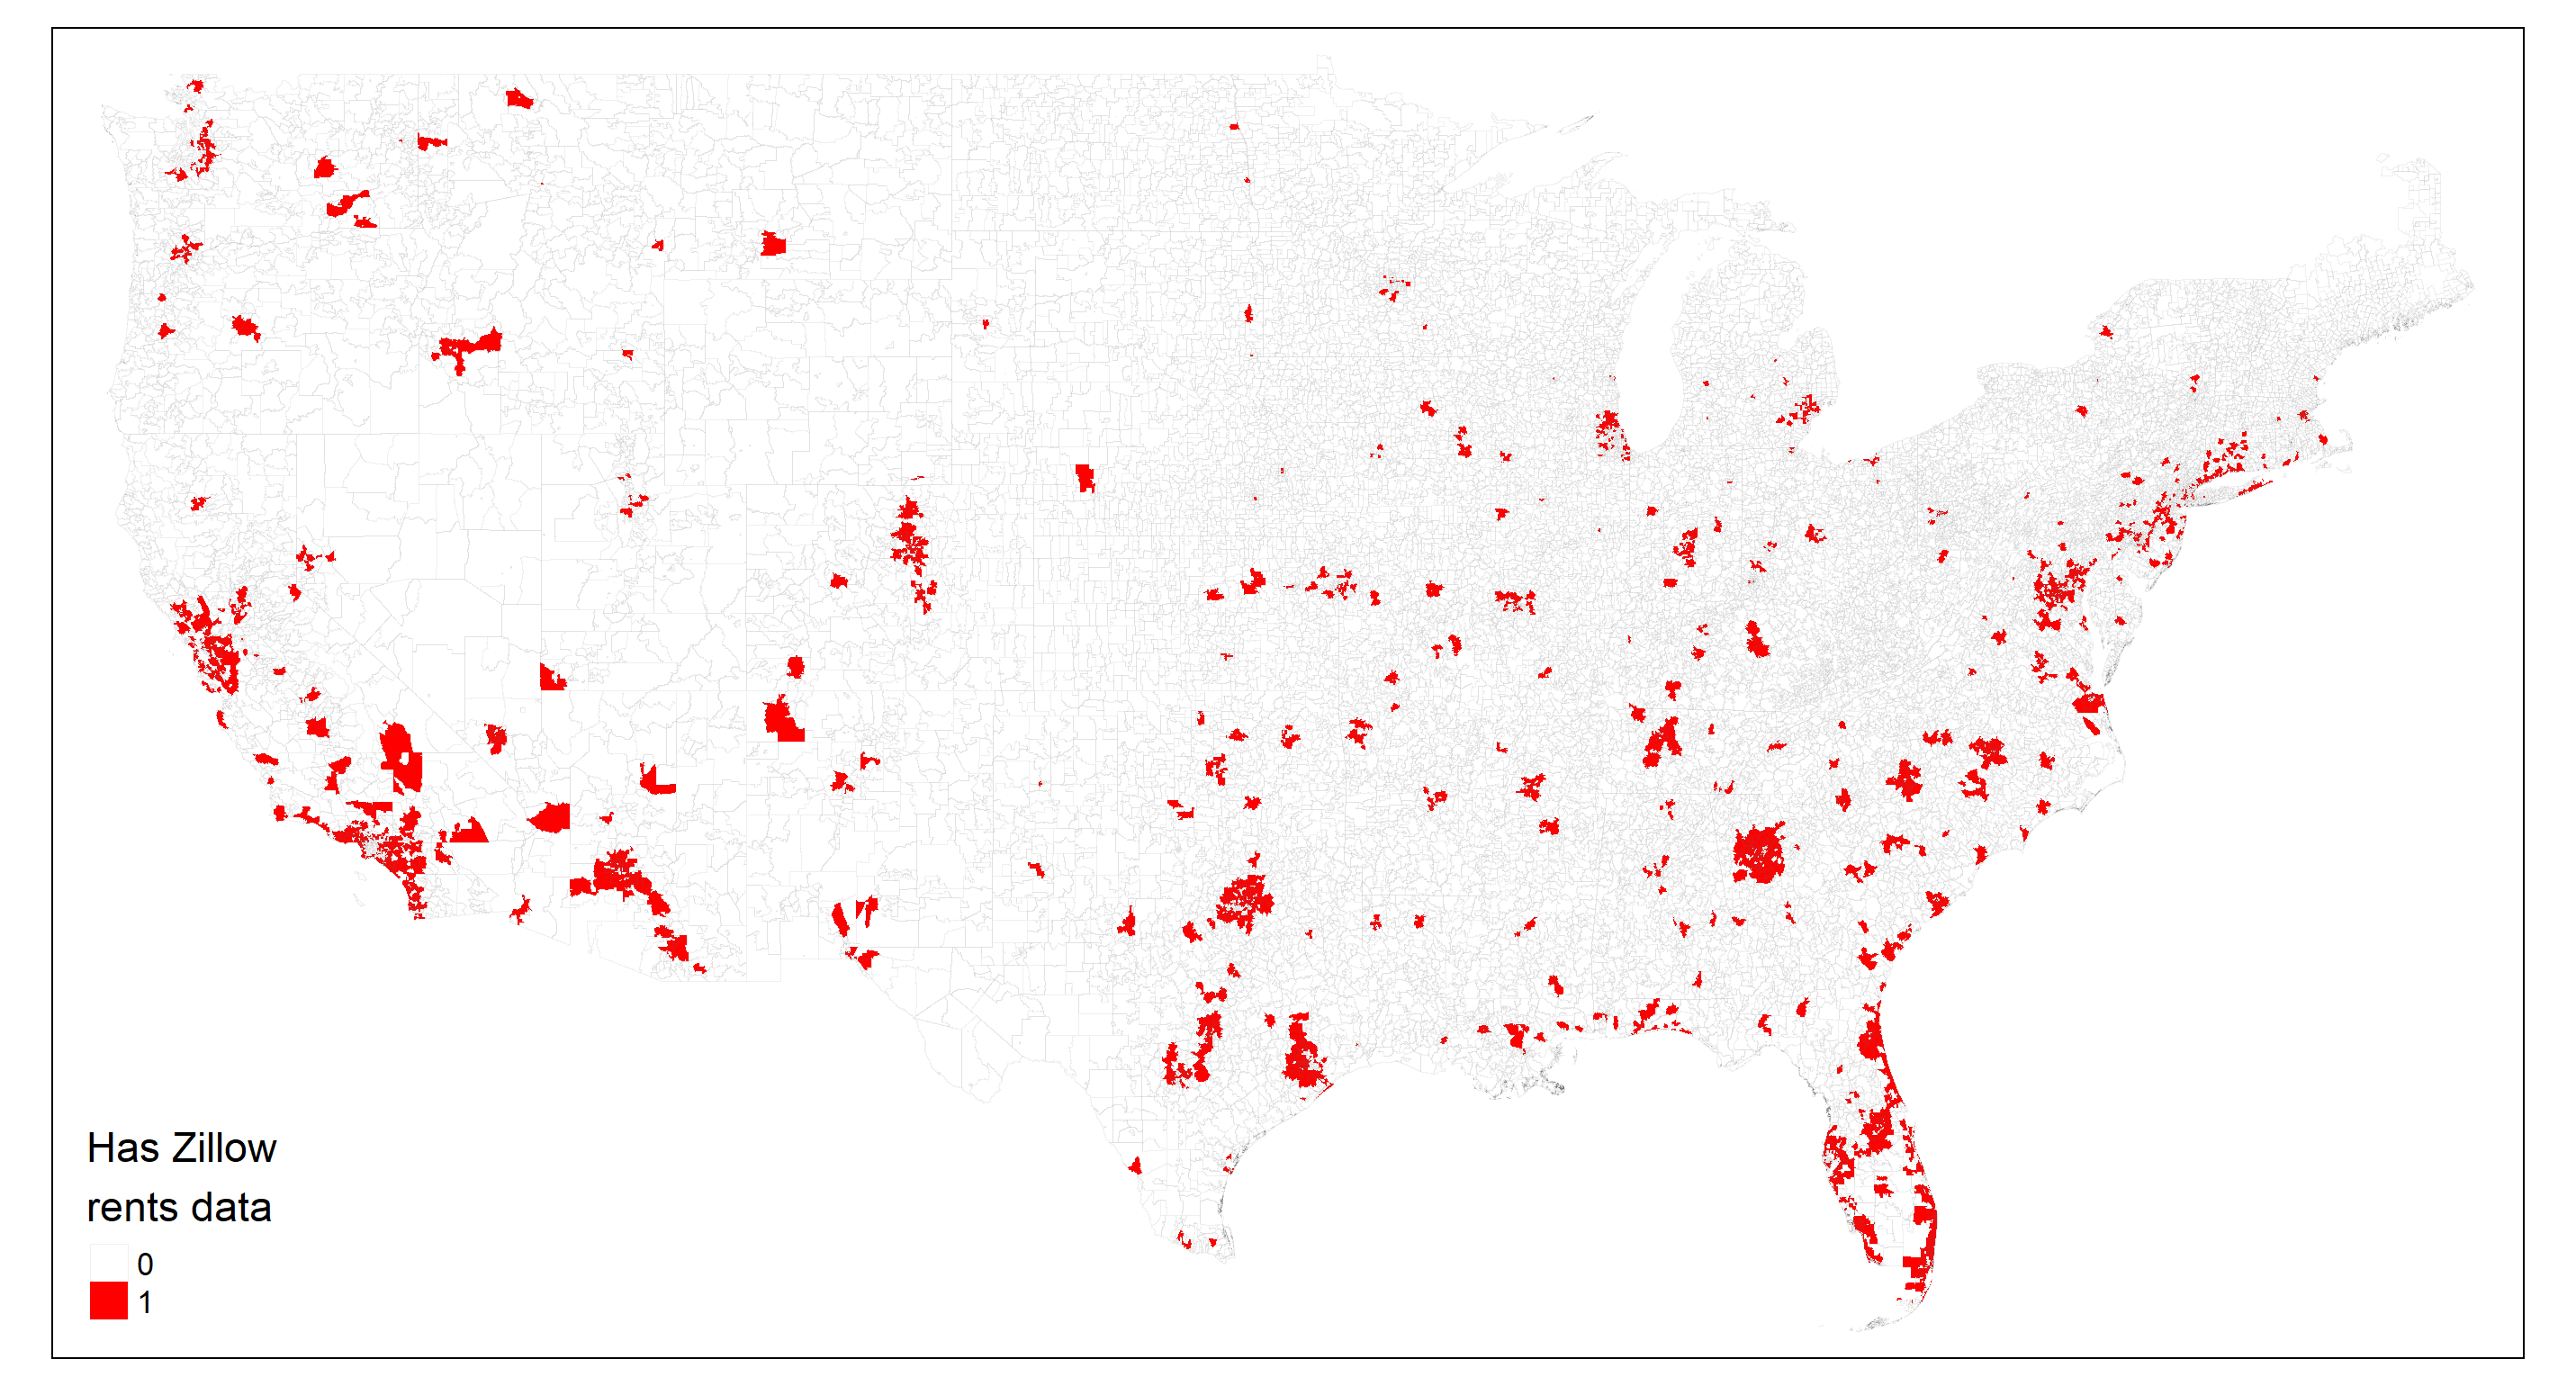
\includegraphics[scale = 0.32]{maps_US/output/USPS_zipcodes_zillow_data.png}
        \end{subfigure}
    \end{figure}
\end{frame}

%\subsection{Minimum Wages}

\begin{frame}[label=stat_MW]
	\frametitle{The Statutory MW}
	
	\begin{itemize}
		\item
		Collect MW data at state, county and city levels between Jan 2010 and Dec 2019.
		
		\vspace{2mm} \item
		Assign those data to ZIP codes.
		
		\vspace{2mm} \item
		Define statutory MW in ZIP code as maximum between state and local levels.
		
		\pause
		\vspace{2mm} \item
		ZIP codes available in Zillow contain 18,689 changes at the ZIP code-month level.
		\vspace{-3.5mm} 
		\begin{itemize} \small
			\item 151 state-level changes.
			\item 182 county- and city-level changes.
		\end{itemize}
		%% We use 4,224 events at the ZIP code-month level in our estimating panel
		
	\end{itemize}
	
\end{frame}

\subsection{Commuting shares}

\begin{frame}
	\frametitle{Using LODES to construct the experienced log MW}
	
	Construct \textbf{origin-destination matrix} at ZIP code level from 2017 LODES.
	%% Original data comes at the block-group level
	Observe:
	\begin{itemize} \small
		\item Number of workers residing in a ZIP code and working in every other 
		ZIP code.
		\item Analogous, matrix for number of workers younger than 29 and earning less than 
		\$1,251.
		%% Exp MW constructed using any of these measures gives similar results
	\end{itemize}
\end{frame}

\subsection{Other Data sources}

\begin{frame}
	\frametitle{Other Data Sources} 
	
	\begin{itemize}
		\item Economic controls from the Quarterly Census of Employment and Wages 
		{\small (QCEW)}.
		\vspace{2mm}  \item IRS Statistics of income - ZIP Code Aggregates (New)
		\vspace{2mm} \item ZIP Code Month panel of rents since 2018 from actual transactions data (New)
	\end{itemize}
\end{frame}

\section{Empirical Strategy}

\subsection{Empirical Models}

\begin{frame}[label = stat_only_model]
	\frametitle{Empirical (Naive) model}
	
	Ignoring the experienced MW, one may estimate the following first differences model:
	
	$$
	\Delta \ln r_{it} = \tilde\delta_t + 
	\tilde\beta \Delta \ln \MW_{it} + 
	\Delta \mathbf{X}^{'}_{c(i)t} \tilde\eta + 
	\Delta \tilde\varepsilon_{it} ,
	$$
	
	where	
	\begin{itemize} \small
	\item ZIP code $i$, county $c(i)$, month $t$;
	
	\item \vspace{1mm} $r_{it}$: rents per square foot;
	
	\item \vspace{1mm} $\ln \MW_{it}$: statutory log MW;
	
	\item \vspace{1mm} $\tilde\delta_t$: month fixed effects (ZIP code FE $\tilde\alpha_i 
	$ is 
	implicit);
	
	\item \vspace{.5mm} $\mathbf{X}_{c(i)t}$: time-varying controls.
	\end{itemize}
\end{frame}

\begin{frame}
	\frametitle{Empirical model}
		
	Now add experienced MW:
	$$
	\Delta \ln r_{it} = \delta_t +
	    \beta {\color{red}\Delta \MW^{\text{exp}}_{it}} +
		\gamma {\color{blue} \Delta \ln \MW_{it}} + 
		\Delta \mathbf{X}^{'}_{c(i)t} \eta + 
		\Delta \varepsilon_{it} ,
	$$
	
	where $\MW^{\text{exp}}_{it}$ is experienced log MW {\small (Recall 
	$\Delta \MW^{\text{exp}}_{it} = \sum_{z \in \mathbb{Z}_i} \pi_{i z} \Delta 
	\ln \MW_{zt}$)}.

	\pause
	\vspace{2mm}
	For causal effect of $\beta$ we need:
	$$
	E \left[\Delta \varepsilon_{ict} {\color{red} \Delta 
	\MW^{\text{exp}}_{ic\tau}} 
	\big| {\color{blue}\Delta \ln \MW_{ict}}, \delta_t, \Delta 
	\mathbf{X}_{ict} \right] = 0
	\quad \quad \forall \tau \in \left[ \underline{T}, \overline{T} \right]
	$$
	
	\pause
	\vspace{2mm}
	\textbf{In words}: conditional on FEs, controls, and {\color{blue} MW in same ZIP 
	code}, unobserved innovations to rent shocks are uncorrelated with past and future 
	values of log MW changes {\color{red} in nearby ZIP codes}.
\end{frame}


\begin{frame}
	\frametitle{Discussion Identification Assumption}
	
	Thus, for causal effect of $\beta$ we need:
	$$
	E \left[\Delta \varepsilon_{ict} \Delta \MW^{\text{exp}}_{ict}  
	\big| \Delta \ln \MW_{ict}, \delta_t, \Delta 
	\mathbf{X}_{ict} \right] = 0
	\quad \quad \forall \tau \in \left[ \underline{T}, \overline{T} \right]
	$$
	\vspace{.5mm}
	Analogously, for causal effect of $\gamma$ we need:
	$$
	E \left[\Delta \varepsilon_{ict} \Delta \ln \MW_{ict}  
	\big| \Delta \MW^{\text{exp}}_{ict}, \delta_t, \Delta \mathbf{X}_{ict} 
	\right] = 0
	\quad \quad \forall \tau \in \left[ \underline{T}, \overline{T} \right]
	$$
	
	\pause
	\vspace{.5mm}
	\textbf{Is this plausible?}
	\begin{itemize} \small
		\vspace{.5mm}
		\item MW policies are rarely set by considering differential dynamics of the 
		rental housing market within metropolitan areas.
		%% For example, the Congressional Budget Office (CBO) doesn't mention rents even 
		%% once in it's study of the effects of the Wage Act of 2021
		%% https://www.cbo.gov/system/files/2021-02/56975-Minimum-Wage.pdf
		
		\vspace{.5mm}
		\item Furthermore, there is substantial heterogeneity in the housing market 
		across ZIP codes.
		
		\vspace{.5mm}
		\item Indirectly test assumption through pre-trends, assuming no anticipatory 
		effects in housing market.
	\end{itemize}
\end{frame}

\begin{frame}[label = dyn_model]
	\frametitle{Testing Identification with a Dynamic model}
	
	Adding leads and lags of the experienced log MW:
	
	$$
	\Delta \ln r_{ict} = \delta_t
		+ \sum_{r=-s}^{s} \beta_r \Delta \MW^{\text{exp}}_{ic,t+r}
		+ \gamma \Delta \ln \MW_{ict}
		+ \Delta \mathbf{X}^{'}_{ct}\eta
		+ \Delta \varepsilon_{ict}
    $$
	
	where $\{\beta_r\}_{r=-s}^{s}$ are the dynamic coefficients.
	
	\vspace{1mm}

    Analogously, one can add instead the leads and lags of the log residence MW
    to test the identification assumption of $\gamma$.
\end{frame}

\section {Identification}

\section{Results}

\subsection{Main Results}

\begin{frame}
    \frametitle{Static }
    
\end{frame}

\begin{frame}
	\begin{figure}
		\centering
		\vspace{-2mm}
		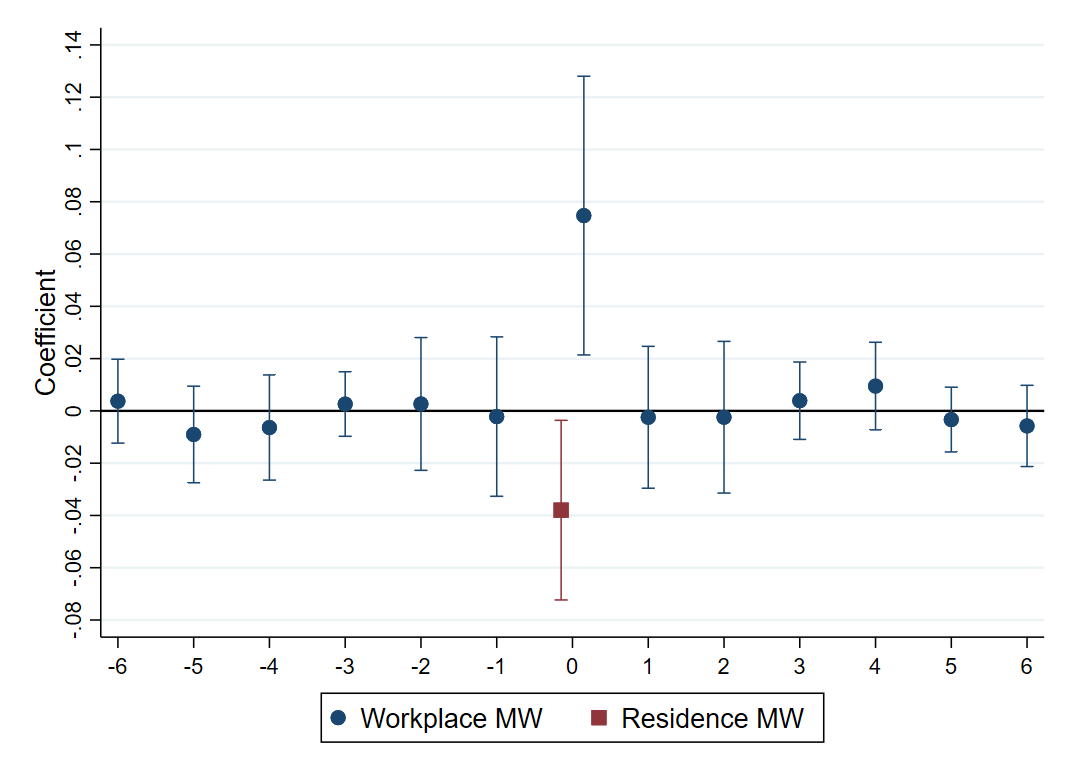
\includegraphics[width=0.8\textwidth]{fd_baseline/output/fd_baseline_exp_ln_mw_17_dynamic.png}
	\end{figure}   
\end{frame}


\section{Robustness and Heterogeneity}

\section{The incidence of counterfactual federal MW change}

\begin{frame}
    \frametitle{Overview}
    
    Entire commuting structure determines the incidence of MW policies.
    \begin{itemize}
    	\vspace{1mm}
    	\item In some ZIP codes both residence and workplace MW increase
    	\vspace{1mm}
    	\item Other nearby ZIP codes are affected only through workplace
    \end{itemize}
    
    \pause
    \vspace{3mm}
    Consider an increase of the federal MW to \$9 in January 2020.
    \begin{itemize}
    	\vspace{1mm}
    	\item Changes income $\{\Delta Y_i\}_{i\in\Z}$ and housing expenditure $\{\Delta H_i\}_{i\in\Z}$
    \end{itemize}
    
    \pause
    \vspace{3mm}
    How much out of each extra dollar is captured by landlords?
   
\end{frame}

\begin{frame}
	\frametitle{Pass-through coefficients}
	Define pass-through coefficients
	
	\begin{equation*}
		\rho_i := \frac{\Delta H_i}{\Delta Y_i} =  \frac{h^{\text{Post}}_i r^{\text{Post}}_i - h^{\text{Pre}}_i r^{\text{Pre}}_i}{\Delta Y_i}
	\end{equation*}
	where 
	\begin{itemize}
		\item $h$ denotes rented space in $i$ (square feet)
		\item Pre and Post indicate moments before and after the increase
	\end{itemize}

	\pause
	\vspace{3mm}
	Change in rented space are unobserved. We assume $h^{\text{Pre}}_i = h^{\text{Post}}_i = h_i$ so
	\begin{equation*}
		\rho_i = \frac{h^{\text{Post}}_i r^{\text{Post}}_i - h^{\text{Pre}}_i r^{\text{Pre}}_i}{\Delta Y_i} = h_i \frac{\Delta r_i}{\Delta Y_i}
	\end{equation*}
	If $\Delta h_i > 0$ then our estimate of $\rho_i$ is a lower bound.

	\pause
	\vspace{2mm}
	We construct empirical analogous of $h_i$, $\Delta r_i$ and $\Delta Y_i$.

\end{frame}

\begin{frame}
    \frametitle{Estimates of total rented space}
       
    We haven't found data on $\{h_i\}$. Therefore we do the following
    
    \begin{itemize}
    	\vspace{1mm}
        \item From Zillow get median rental price $R_i$ and median rental price per square foot $r_i$
        \vspace{1mm}
        \item Estimate average square footage $q_i = \frac{R_i}{r_i}$
        \vspace{1mm}
        \item Compute number of rented units $N_i$ from ACS 2019
    \end{itemize}
    
    \pause
    \vspace{3mm}
    Our estimates of total rented space in each ZIP code $i$ are
    \[
    \hat h_i = q_i N_i
    \]
\end{frame}

\begin{frame}
    \frametitle{Model-based estimates of rent changes}
    
    Increase in federal MW to \$9 generates $\{\Delta \hat{\ln \MW}_i\}_{i\in\Z}$
    \begin{itemize}
    	\item $\Delta \hat{\ln \MW}_i=0$ for ZIP codes with binding MWs above \$9
    \end{itemize}
    
    \pause
	\vspace{3mm}
	We proceed as follows
	\vspace{1mm}
	\begin{itemize}
		\item Estimate $\{\Delta \ln r_i\}$ using our baseline model
		\begin{equation*}
			\Delta \hat{\ln r_i} = \gamma \Delta \hat{\ln \MW}_i + \beta \sum_{z\in\Z_i} \pi_{iz} \Delta \hat{\ln \MW}_z
		\end{equation*}
		\item Using $r^{\text{Pre}}_i$ from Zillow as of December 2019, compute 
		$$\Delta \hat r_i = \left(\exp(\Delta \hat{\ln r_i}) - 1 \right) r_i^{\text{Pre}}$$
	\end{itemize}

\end{frame}

\begin{frame}
	\frametitle{Model-based estimates of income changes}
	
	Increase in federal MW to \$9 generates $\{\Delta \hat{\ln \MW}_i\}_{i\in\Z}$
	
	\pause
	\vspace{3mm}
	We need an elasticity of income to the MW $\epsilon$
	\begin{itemize}
		\item Estimate new model using IRS data, obtains $0.14$ [BUTTON TO RESULTS]
		\vspace{1mm} 
		\item Use estimates from the literature \parencite{CegnizEtAl2019}
	\end{itemize}

	\pause
	\vspace{3mm}
	We proceed as follows
	\begin{itemize}
		\item Use elasticity $\epsilon$ to get
		\begin{equation*}
			\Delta \hat{\ln Y}_i = \epsilon \sum_{z\in\Z_i} \pi_{iz} \Delta \hat{\ln \MW}_i
		\end{equation*}
		\vspace{1mm} 
		\item Compute $\Delta \hat Y_i$ using $Y_i^{\text{Pre}}$ as of 2018
		$$\Delta \hat Y_i = \left(\exp(\Delta \hat{\ln Y_i}) - 1 \right) Y_i^{\text{Pre}}$$
	\end{itemize}
\end{frame}

\begin{frame}
	\frametitle{The incidence of MW changes across space}
	
	Figure distribution here
\end{frame}

\begin{frame}[c]
    \begin{center}
    	\Large Thank You!
    \end{center}
\end{frame}

%%%%%%%%%%%%%%%%%%%%%%%%%%%%%%%%%%%%%%%%%%%%%%%%%%%%%%%%%%%%%%%%%%%%%%%%%%%%%%%%%%%%%%%%%%
%                                       APPENDIX                                        %
%%%%%%%%%%%%%%%%%%%%%%%%%%%%%%%%%%%%%%%%%%%%%%%%%%%%%%%%%%%%%%%%%%%%%%%%%%%%%%%%%%%%%%%%%%

\appendix

\renewcommand\thetable{\thesection.\arabic{table}} 
\renewcommand\thefigure{\thesection.\arabic{figure}} 
\setcounter{table}{0}
\setcounter{figure}{0}

\section{Appendix}

\begin{frame}[label = nyc_example]
\frametitle{Other examples: New York (MW Changes in January 2019)}
    \begin{columns}
        \begin{column}{0.50\textwidth}
            \vspace{-4mm}
            \begin{figure}
                \centering
                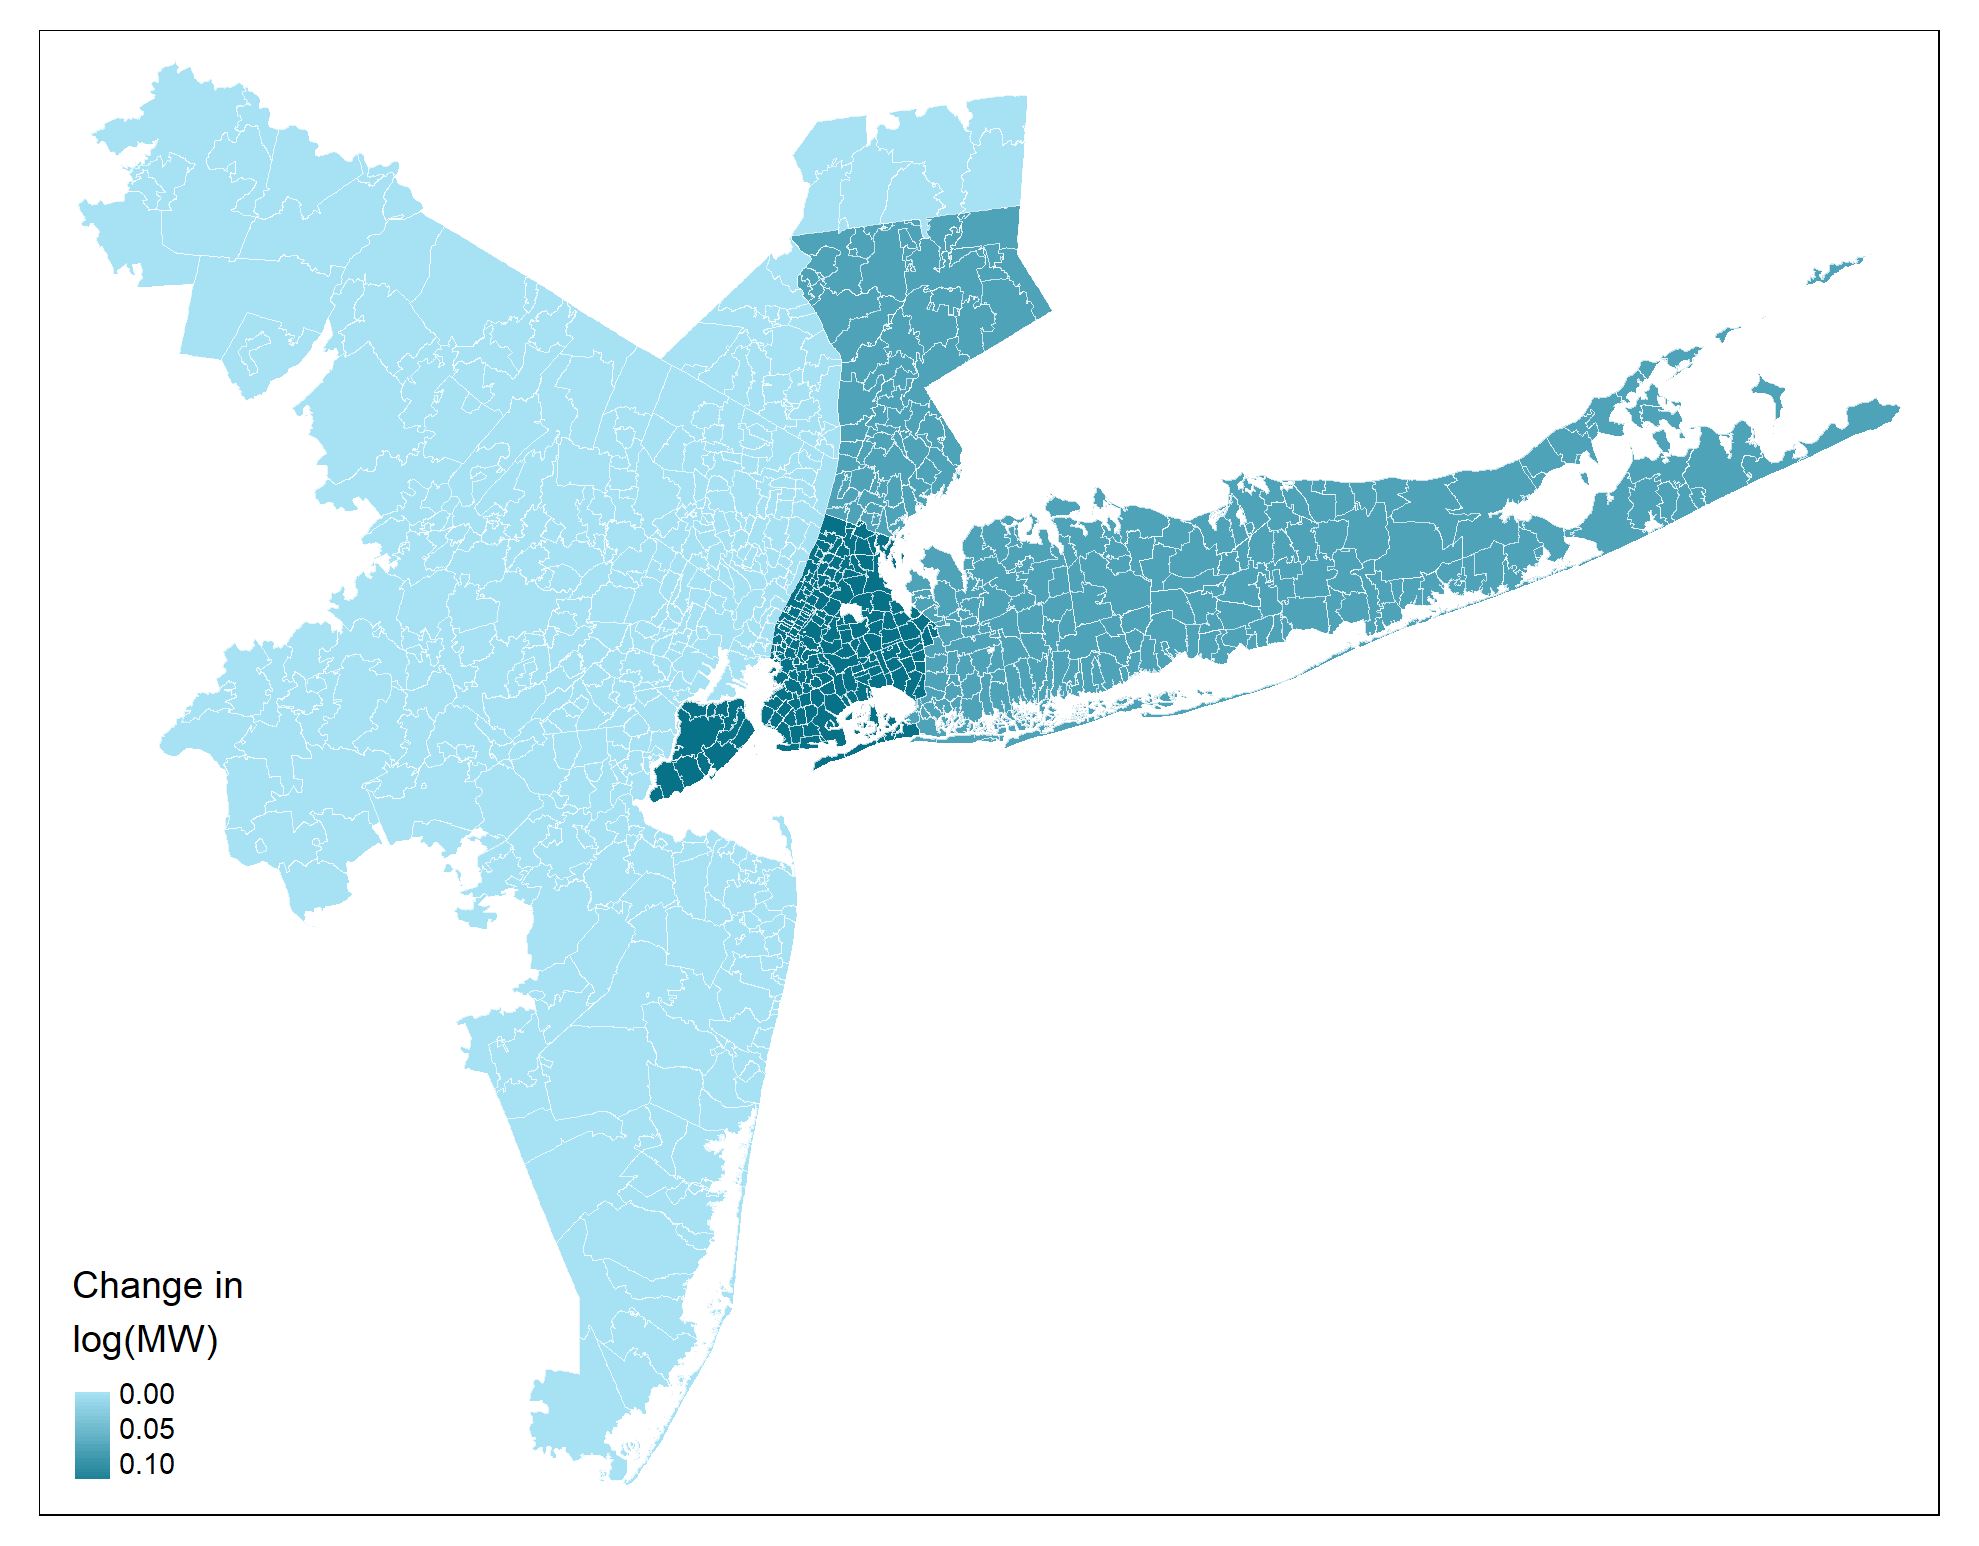
\includegraphics[scale = 0.36]{../../../analysis/maps_events/output/nyc_2018-12_actual_mw.png}
            \end{figure}   
        \end{column}
        \begin{column}{0.50\textwidth}
            \vspace{-4mm}
            \begin{figure}
                \centering
                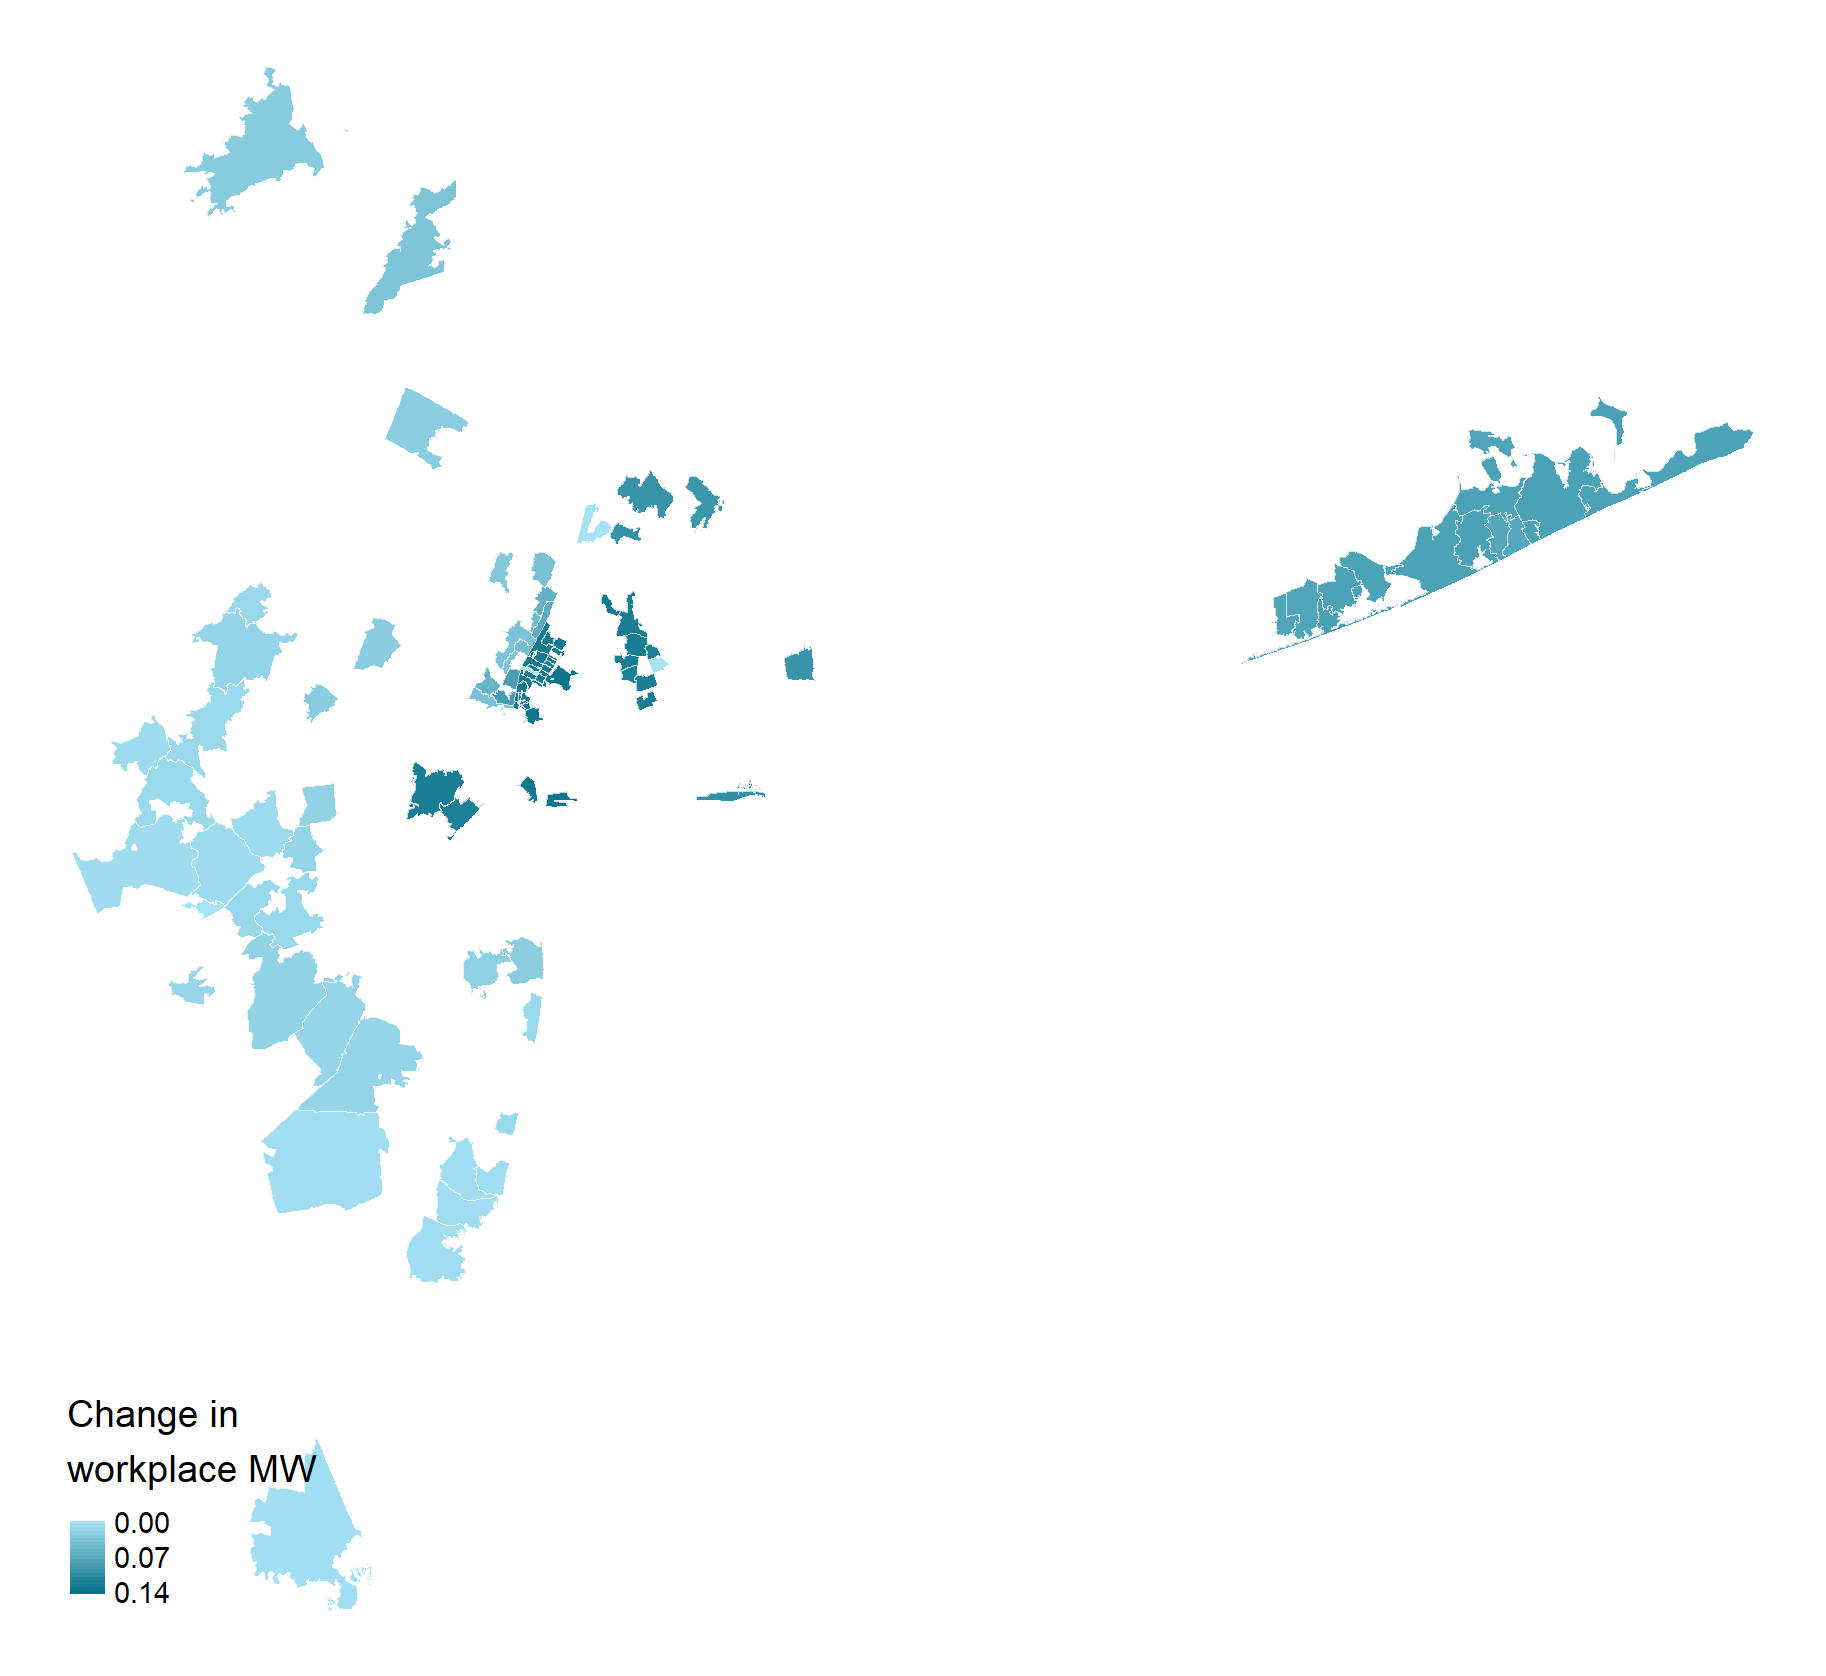
\includegraphics[scale = 0.36]{../../../analysis/maps_events/output/nyc2018-12_exp_mw.png}
            \end{figure}   
        \end{column}
    \end{columns}
    \hyperlink{chi_example}{\beamerbutton{Go back}}
\end{frame}

\begin{frame}[label = bay_example]
\frametitle{Other examples: Bay area (MW Changes in January 2019)}
    \begin{columns}
        \begin{column}{0.50\textwidth}
            \vspace{-4mm}
            \begin{figure}
                \centering
                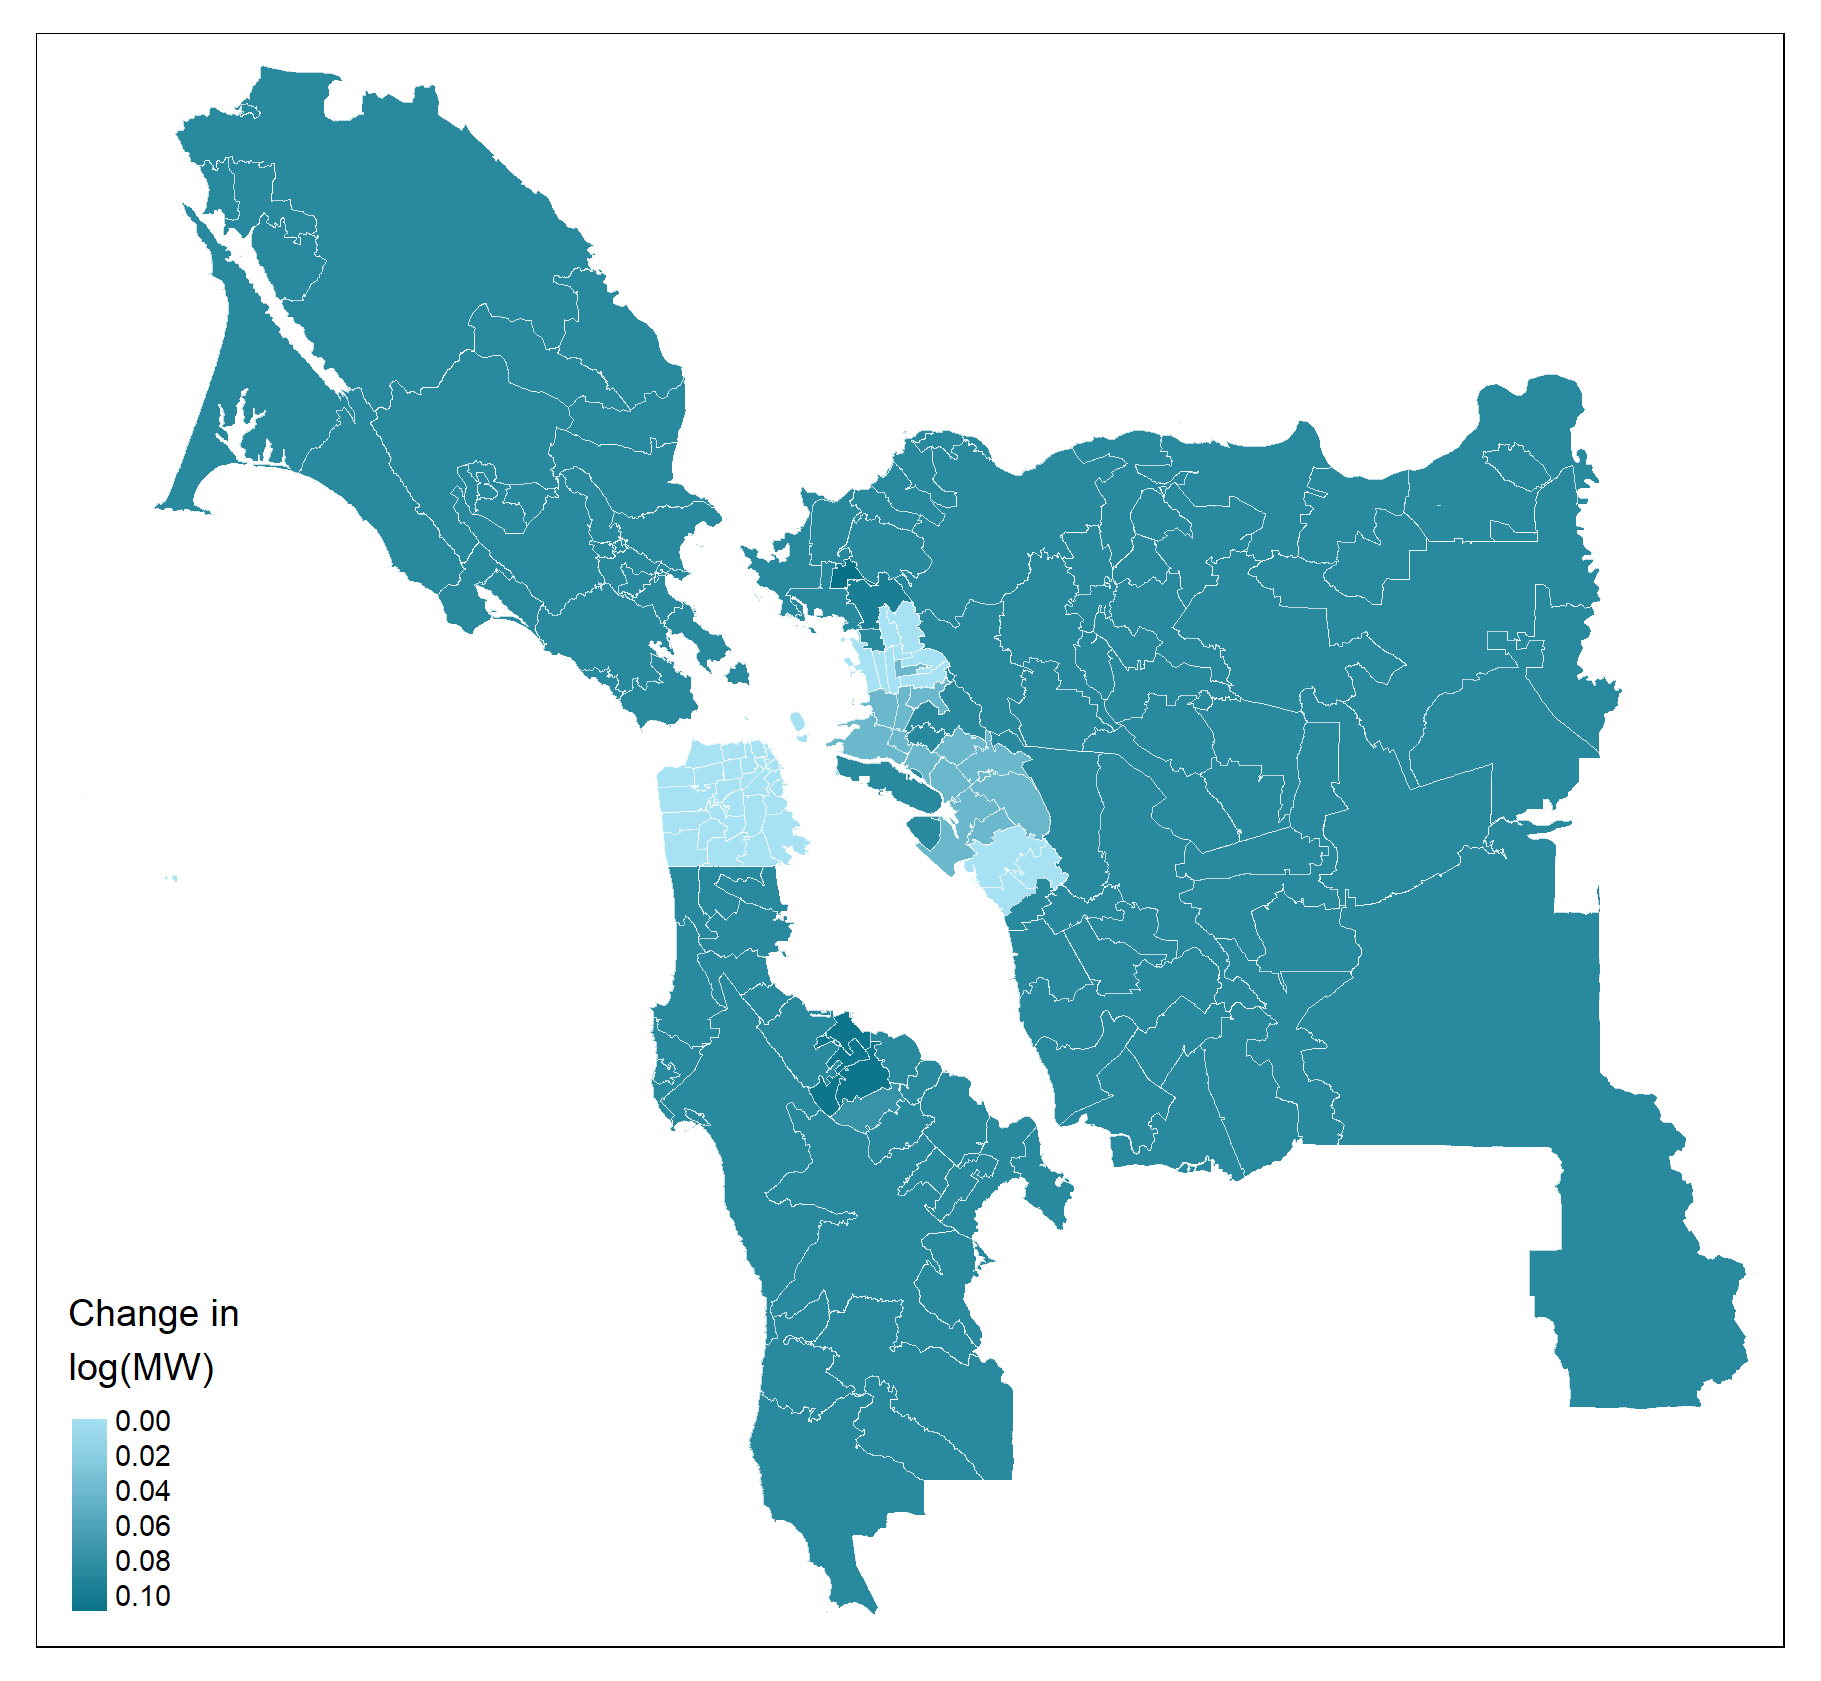
\includegraphics[scale = 0.36]{../../../analysis/maps_events/output/bay_area_2018-12_actual_mw.png}
            \end{figure}   
        \end{column}
        \begin{column}{0.50\textwidth}
            \vspace{-4mm}
            \begin{figure}
                \centering
                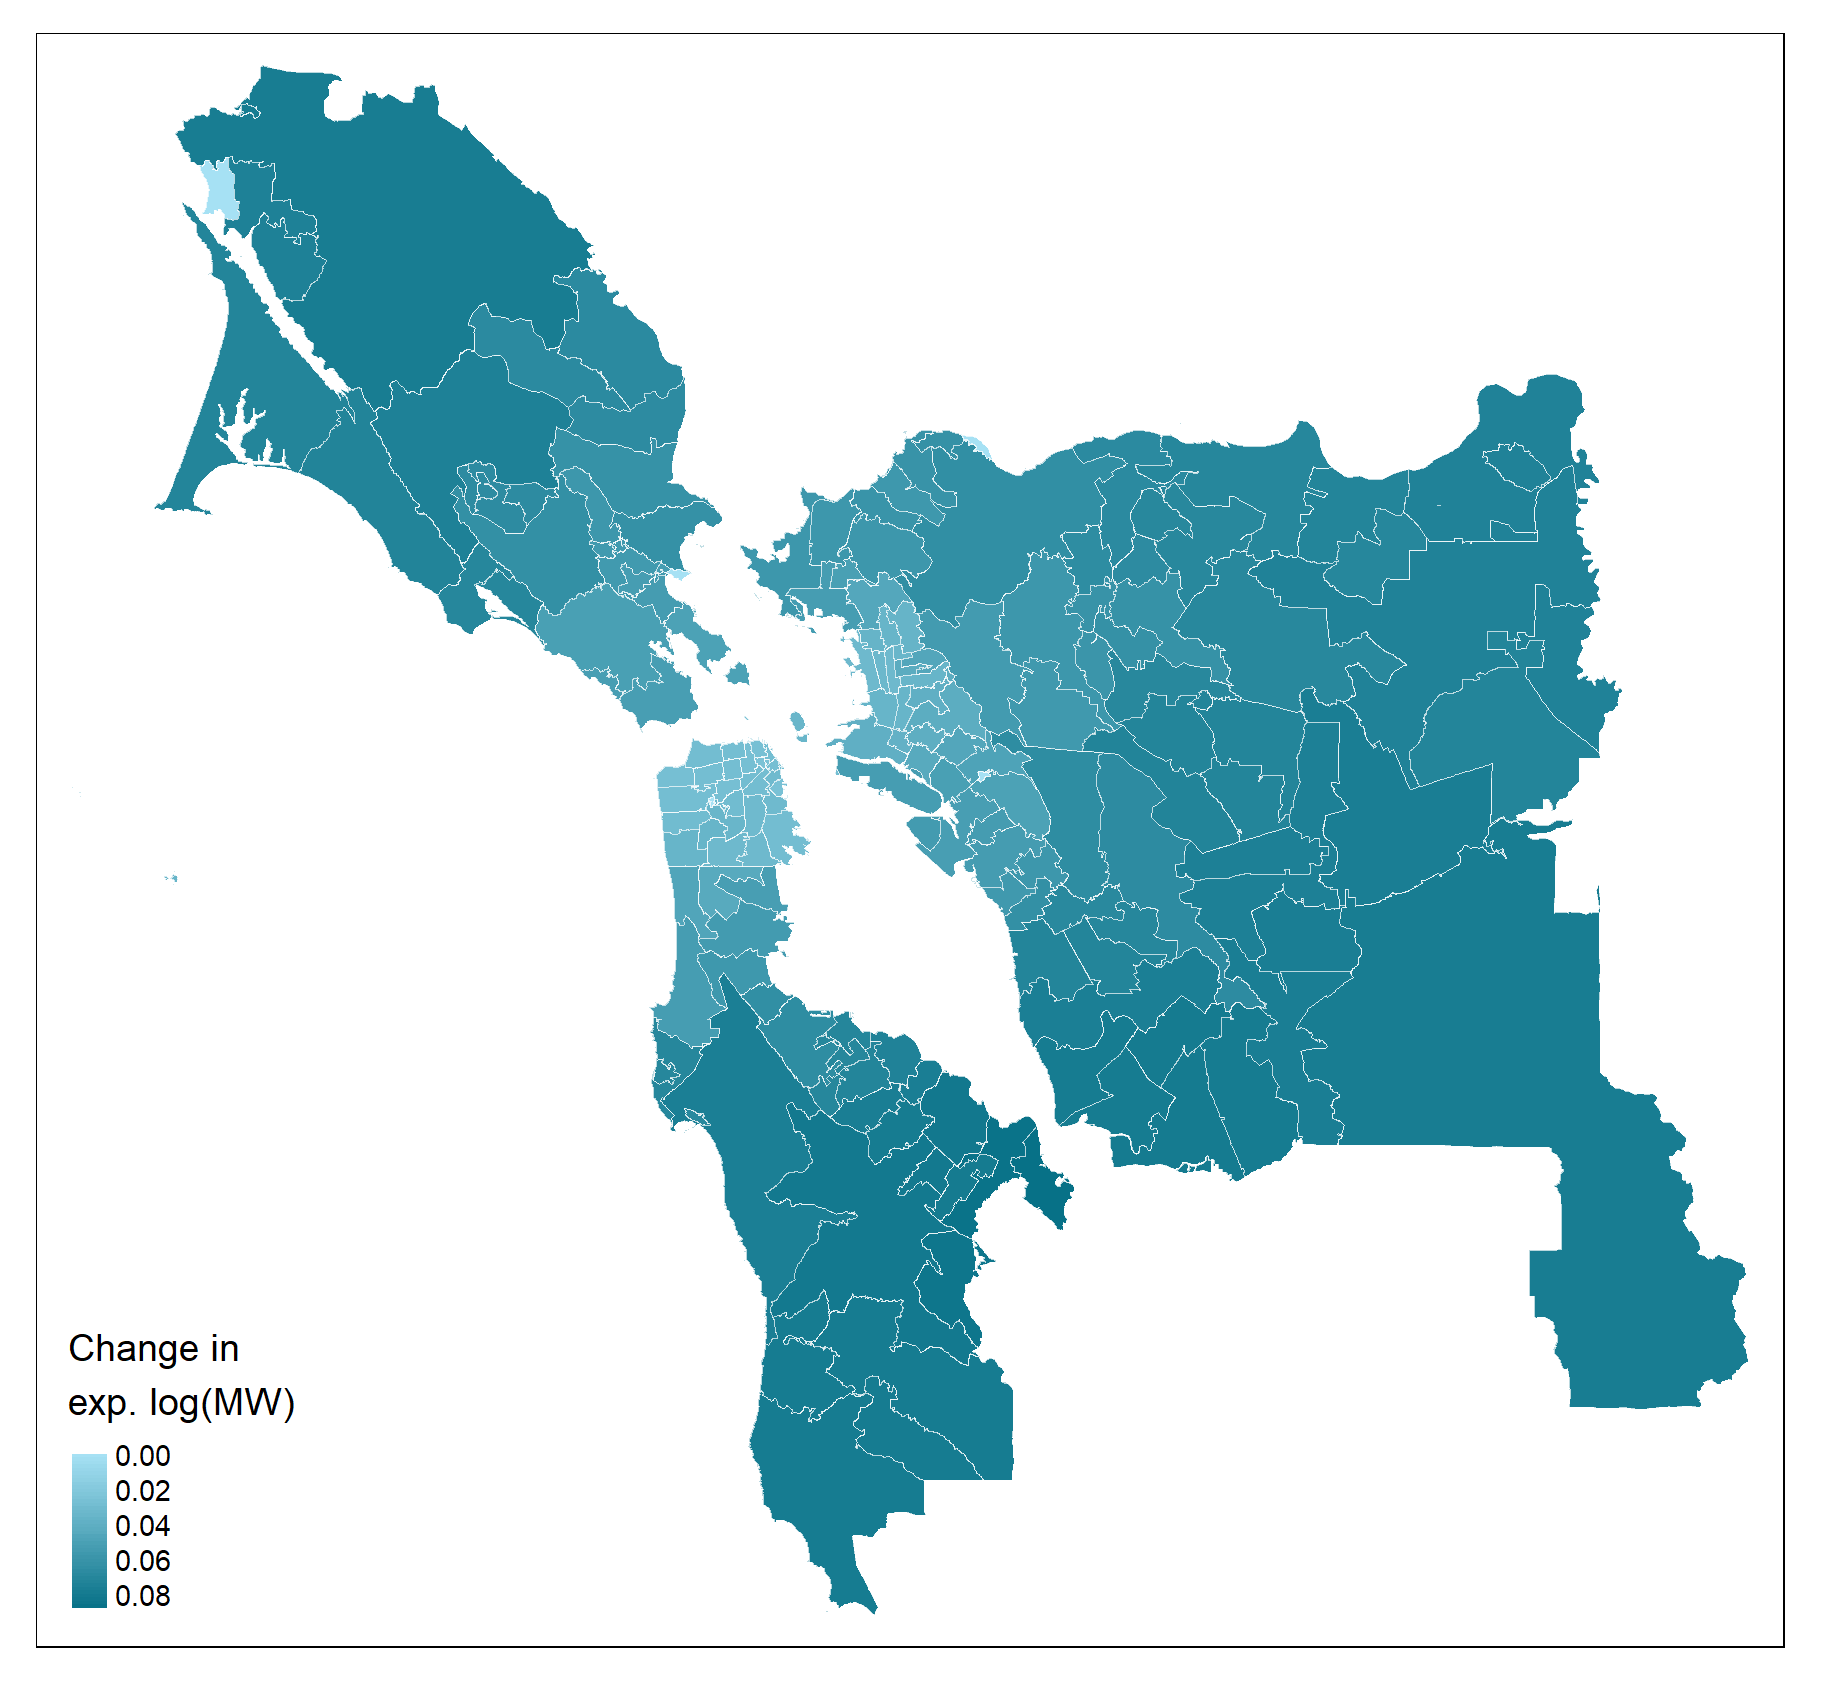
\includegraphics[scale = 0.36]{../../../analysis/maps_events/output/bay_area2018-12_exp_mw.png}
            \end{figure}   
        \end{column}
    \end{columns}
    \hyperlink{chi_example}{\beamerbutton{Go back}}
\end{frame}

\begin{frame}[label = seattle_example]
\frametitle{Other examples: Seattle (MW Changes in January 2018)}
    \begin{columns}
        \begin{column}{0.50\textwidth}
            \vspace{-4mm}
            \begin{figure}
                \centering
                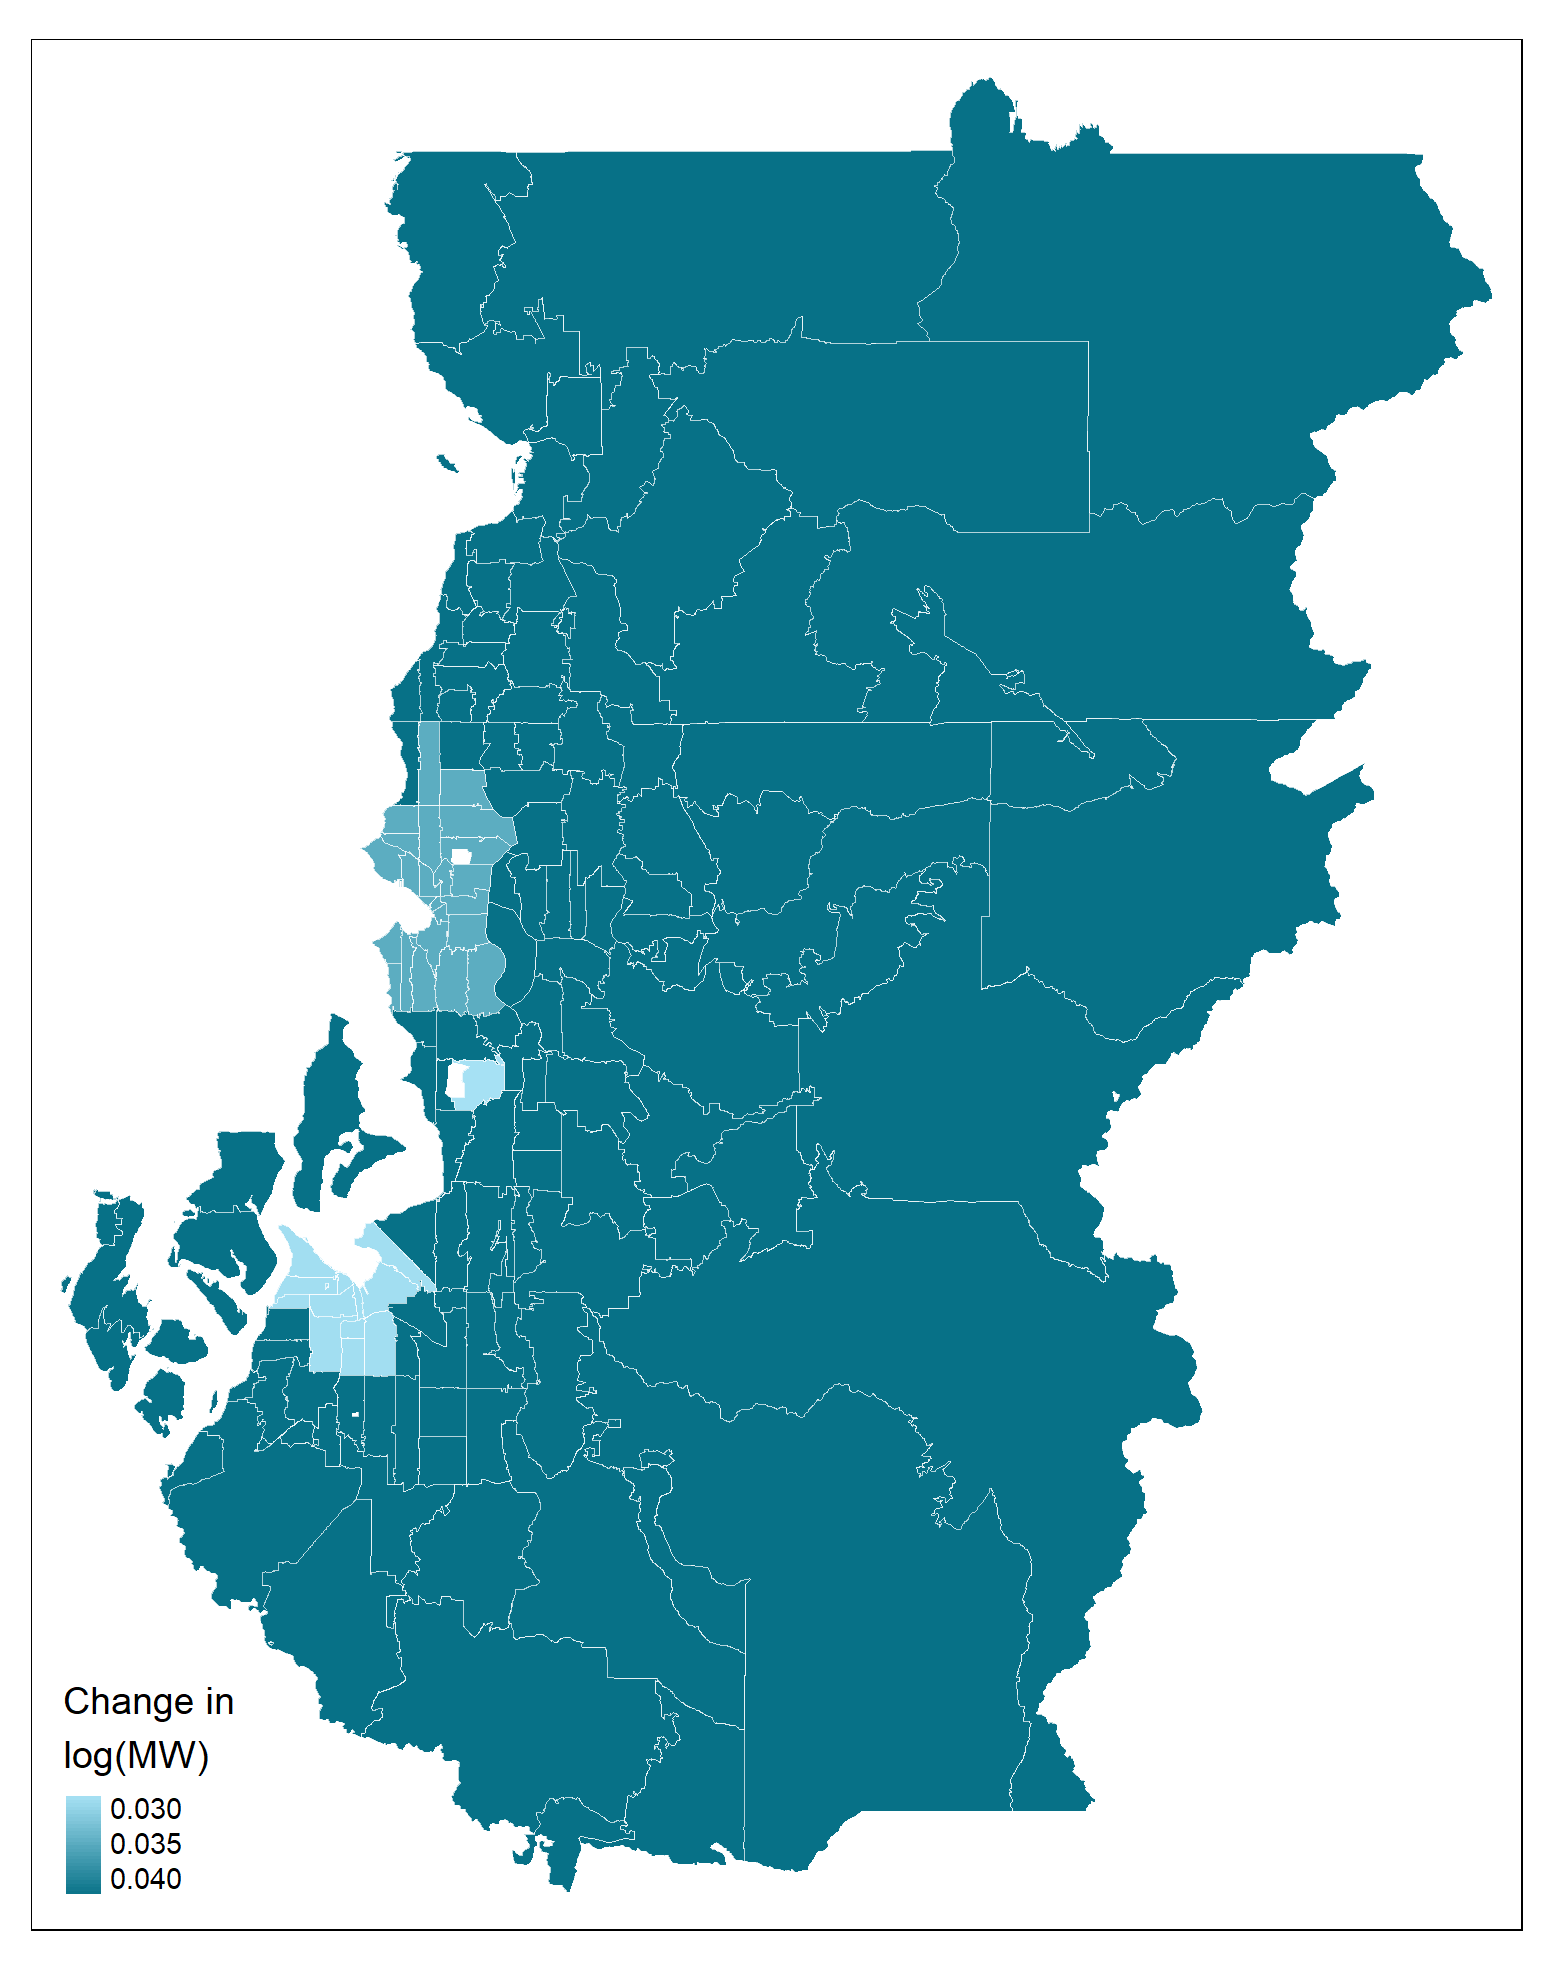
\includegraphics[scale = 0.36]{../../../analysis/maps_events/output/seattle_2018-12_actual_mw.png}
            \end{figure}   
        \end{column}
        \begin{column}{0.50\textwidth}
            \vspace{-4mm}
            \begin{figure}
                \centering
                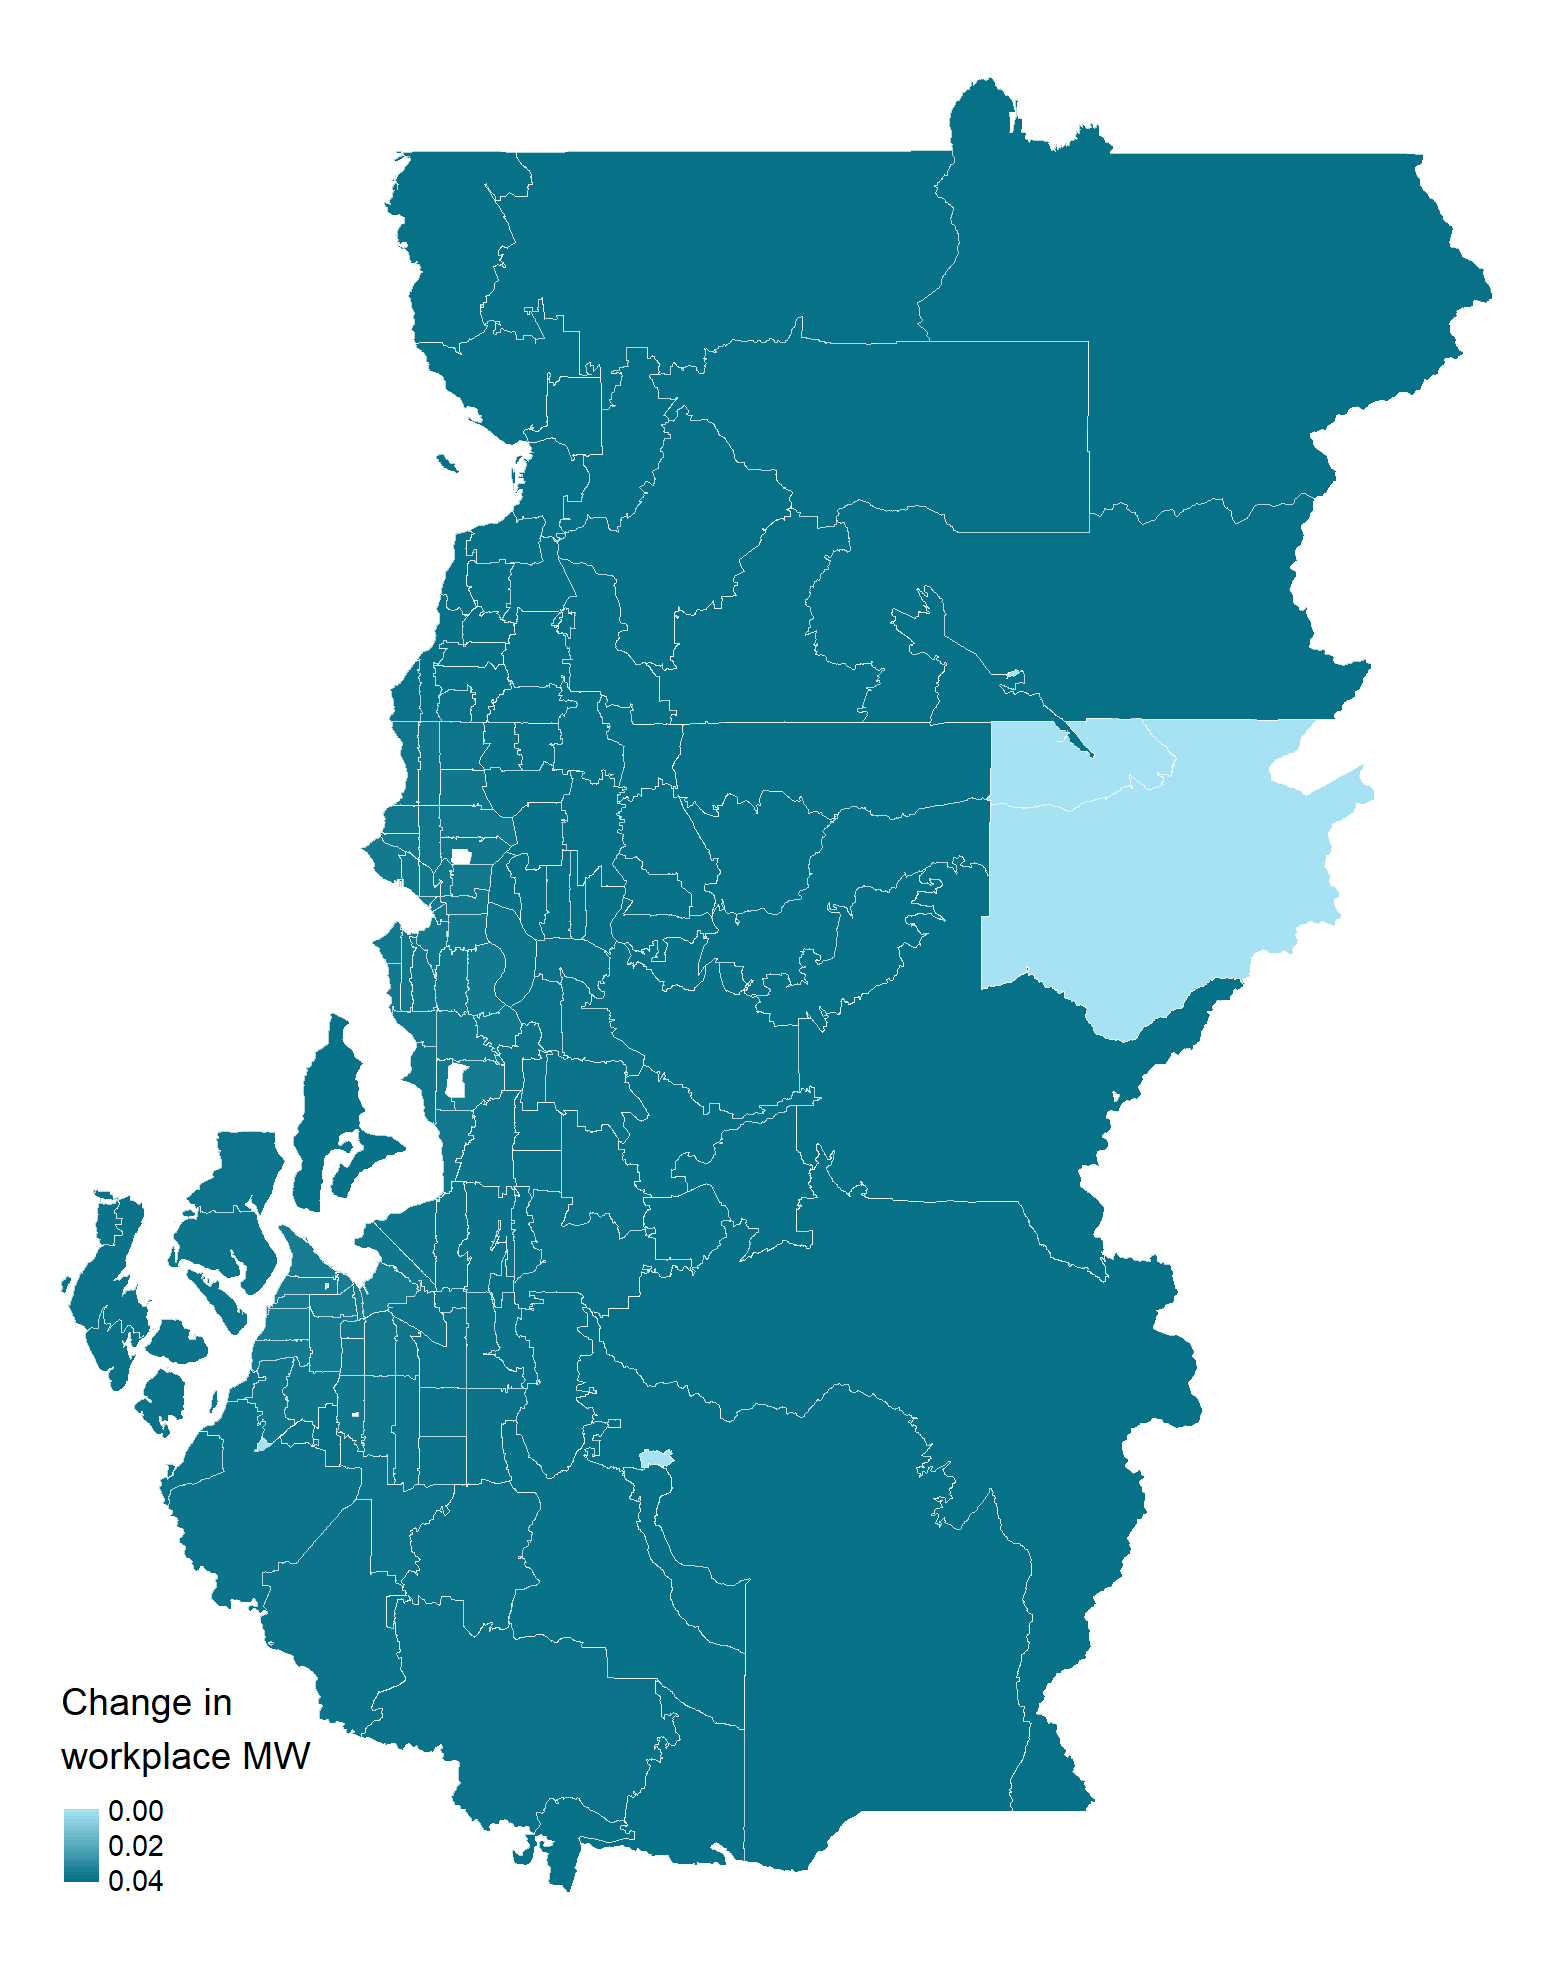
\includegraphics[scale = 0.36]{../../../analysis/maps_events/output/seattle2018-12_exp_mw.png}
            \end{figure}   
        \end{column}
    \end{columns}
     \hyperlink{chi_example}{\beamerbutton{Go back}}
\end{frame}

\begin{frame}[label = san_diego_example]
\frametitle{Other examples: San Diego (MW Changes in January 2019)}
    \begin{columns}
        \begin{column}{0.50\textwidth}
            \vspace{-4mm}
            \begin{figure}
                \centering
                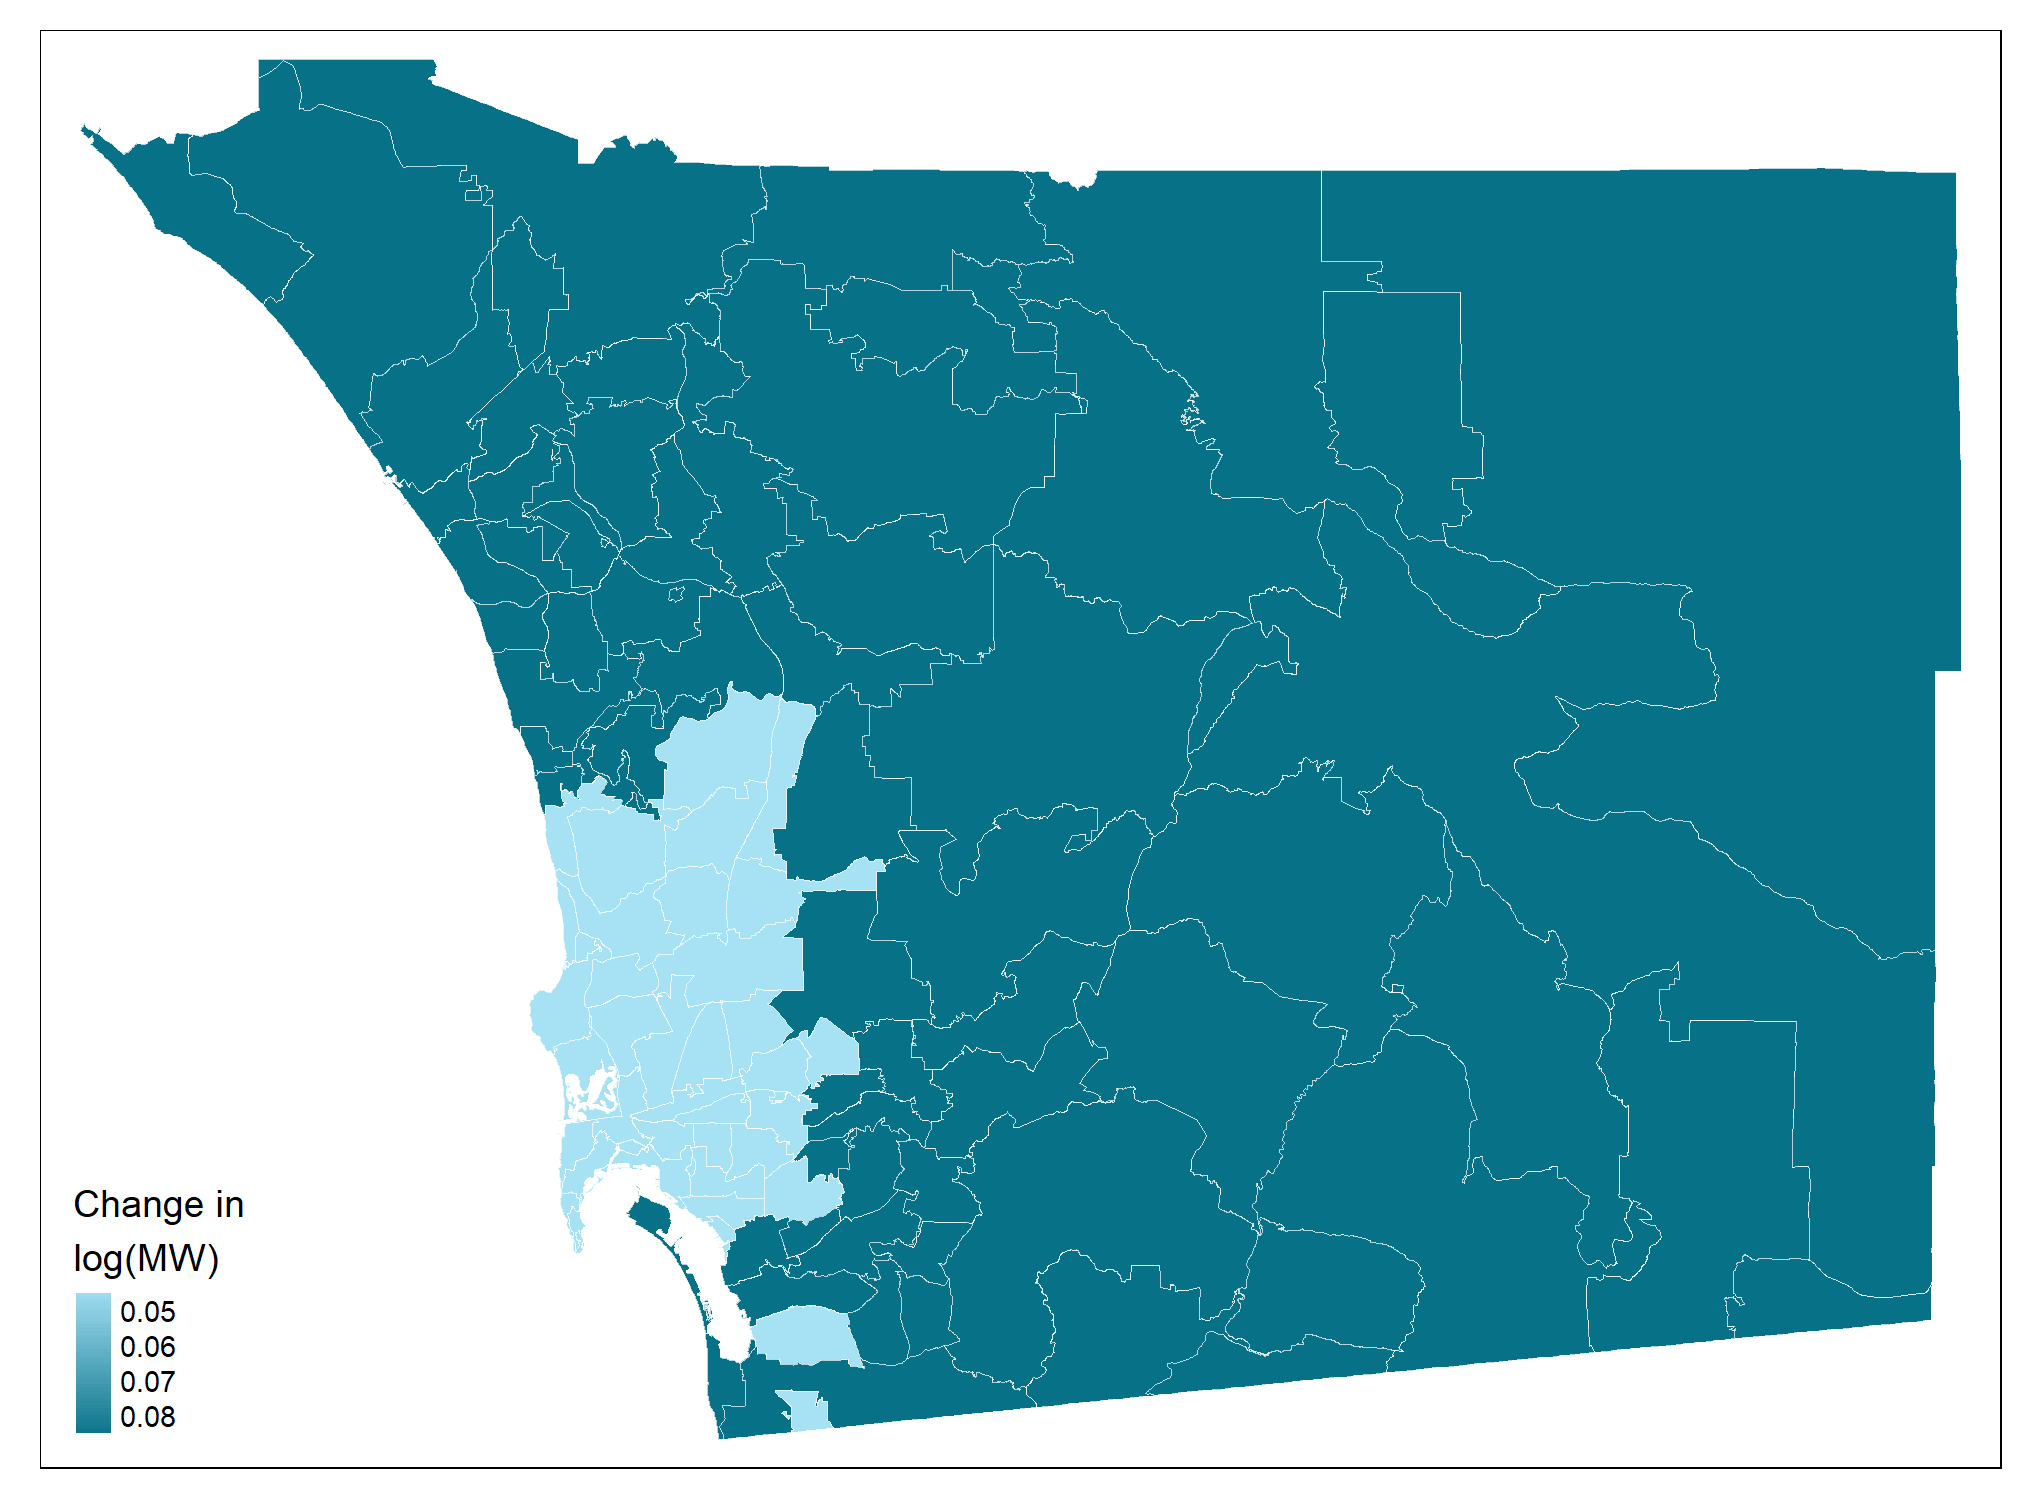
\includegraphics[scale = 0.36]{../../../analysis/maps_events/output/san_diego_2018-12_actual_mw.png}
            \end{figure}   
        \end{column}
        \begin{column}{0.50\textwidth}
            \vspace{-4mm}
            \begin{figure}
                \centering
                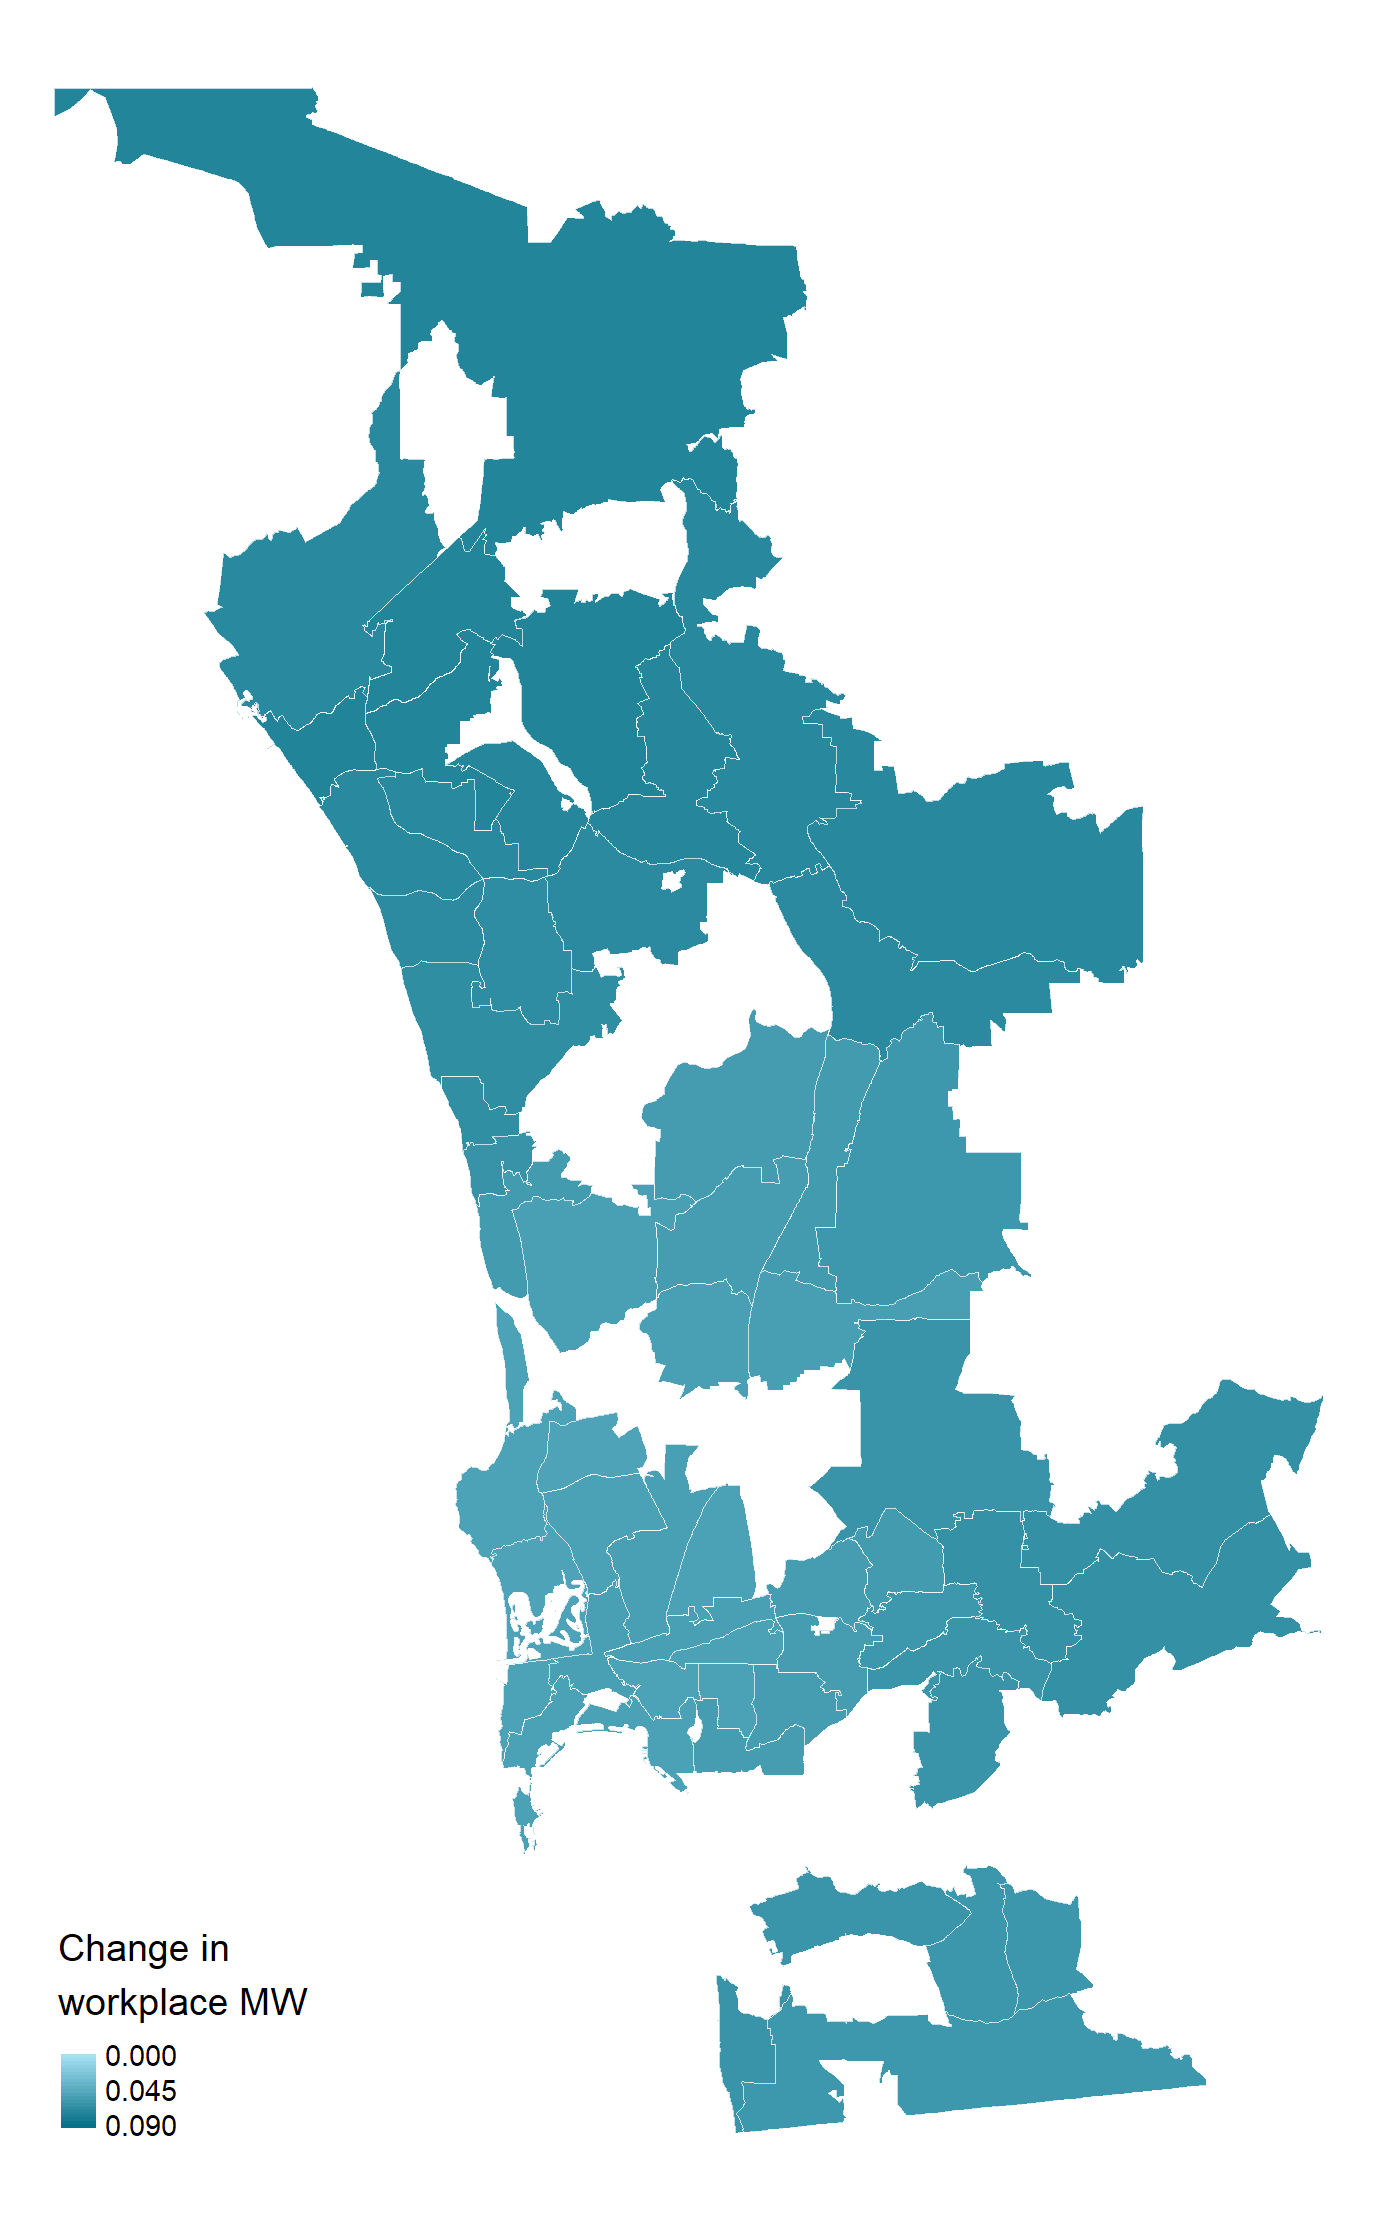
\includegraphics[scale = 0.36]{../../../analysis/maps_events/output/san_diego2018-12_exp_mw.png}
            \end{figure}   
        \end{column}
    \end{columns}
     \hyperlink{chi_example}{\beamerbutton{Go back}}
\end{frame}

\begin{frame}[label = kc_example]
\frametitle{Other examples: Kansas City (MW Changes in January 2019)}
    \begin{columns}
        \begin{column}{0.50\textwidth}
            \vspace{-4mm}
            \begin{figure}
                \centering
                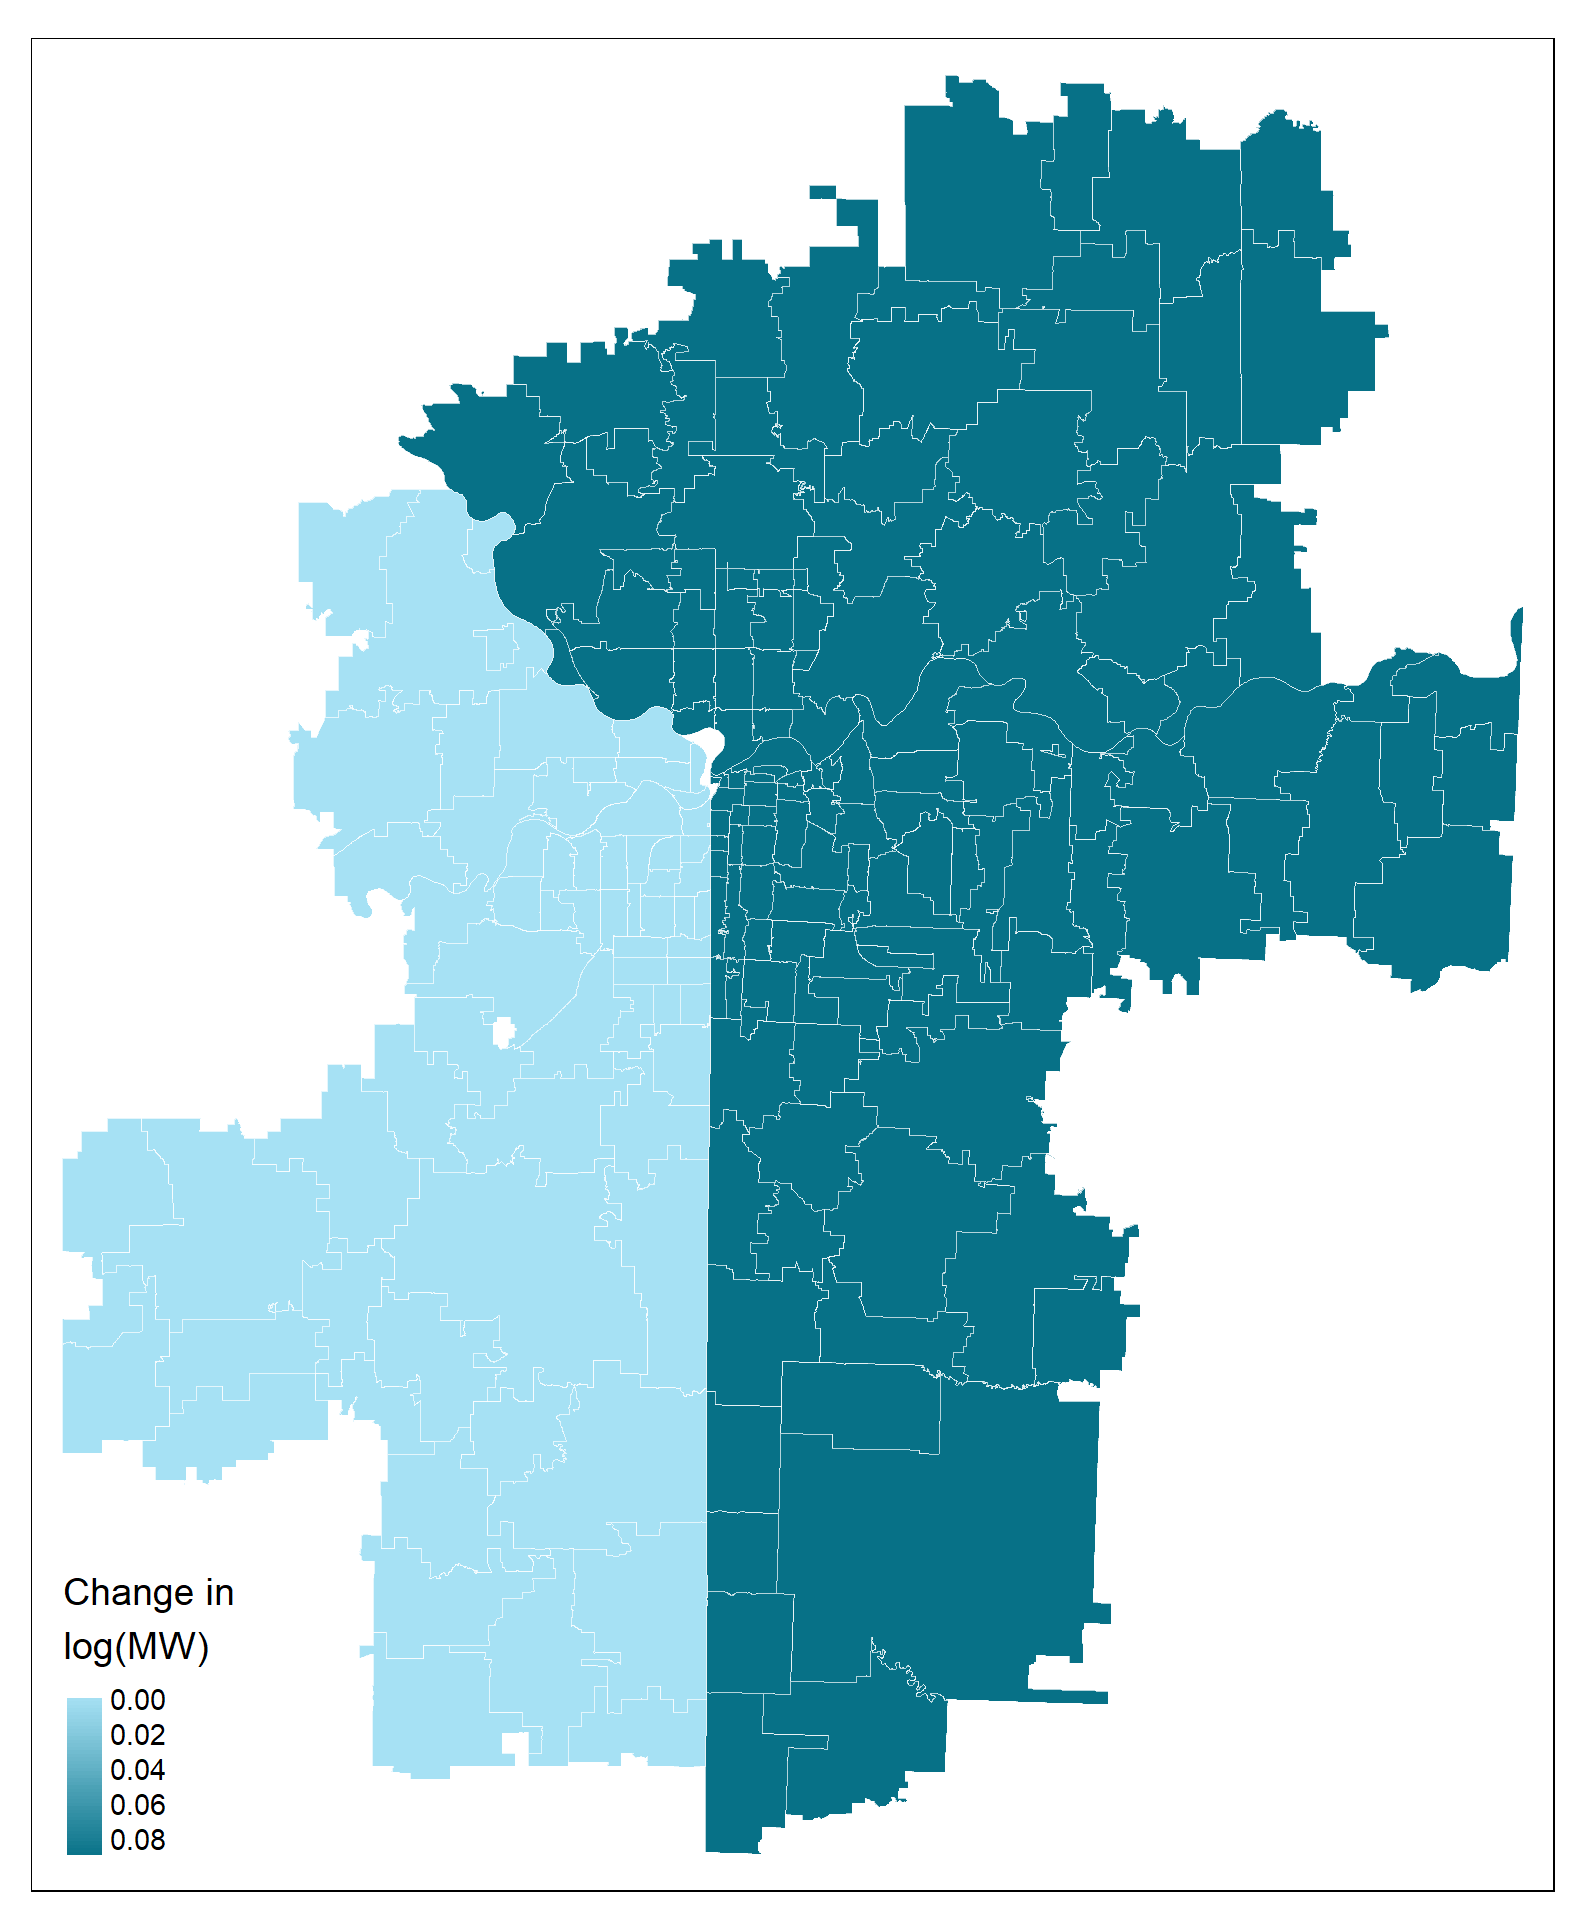
\includegraphics[scale = 0.36]{../../../analysis/maps_events/output/kc_2018-12_actual_mw.png}
            \end{figure}   
        \end{column}
        \begin{column}{0.50\textwidth}
            \vspace{-4mm}
            \begin{figure}
                \centering
                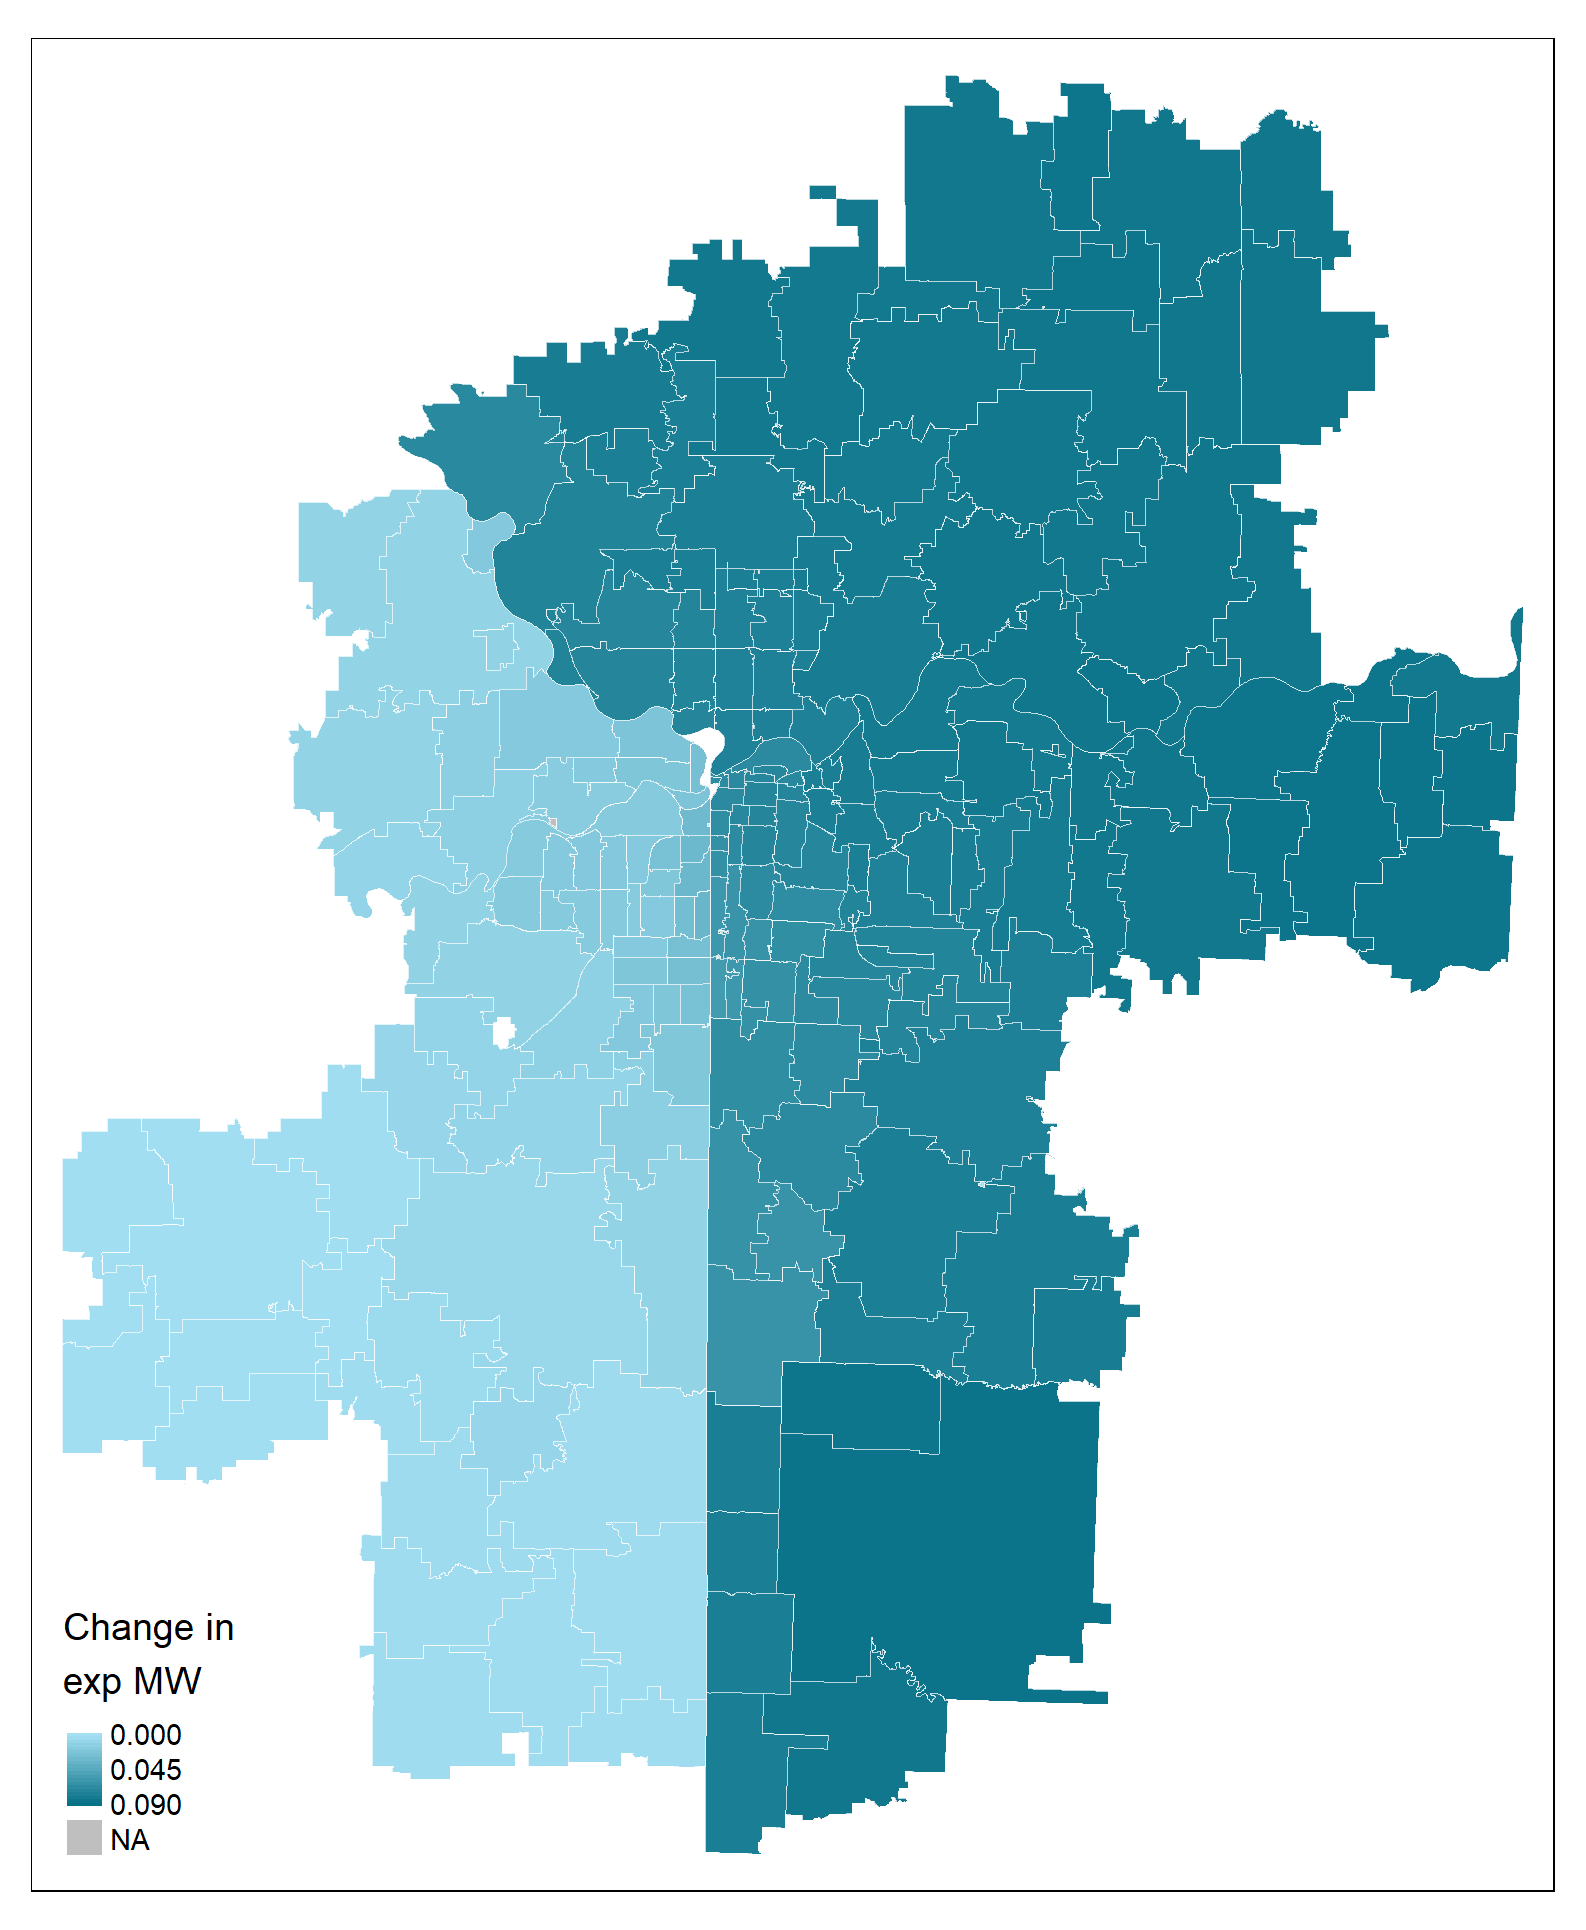
\includegraphics[scale = 0.36]{../../../analysis/maps_events/output/kc2018-12_exp_mw.png}
            \end{figure}   
        \end{column}
    \end{columns}
     \hyperlink{chi_example}{\beamerbutton{Go back}}
\end{frame}

\end{document}